\documentclass[12pt,a4paper,titlepage]{scrartcl}
\usepackage[utf8]{inputenc}
\usepackage[T1]{fontenc}
\usepackage[ngerman]{babel}
\renewcommand{\rmdefault}{ppl}
\renewcommand{\sfdefault}{pfr}
\usepackage{amsmath}
\usepackage{amsfonts}
\usepackage{amssymb}
\usepackage{pifont}


%Seitelayout bearbeiten
\usepackage[paper=a4paper,left=30mm,right=25mm,top=25mm,bottom=25mm, headsep=5mm, headheight=20mm, footskip=10mm]{geometry}
%Zeilenabstand
\usepackage[onehalfspacing]{setspace}

%um Grafiken und Bilder einzufügen
\usepackage{graphicx}
\usepackage{xcolor}
\usepackage{transparent}
\usepackage{pgf}
\usepackage{pgfplots}
\usepackage{pgffor}
\usepgflibrary{plothandlers}
\usepackage{epstopdf}

\graphicspath{{../Bilder/}}
\setlength\intextsep{18.0pt plus 2.0pt minus 2.0pt}
\setlength\textfloatsep{12.0pt plus 2.0pt minus 2.0pt}

\usepackage{caption}
\usepackage{subcaption}

\definecolor{OliveGreen}{rgb}{0,0.6,0}
\newcommand{\cmark}{\Large{\color{OliveGreen}\ding{51}}\normalsize}
\newcommand{\xmark}{\Large{\color{red}\ding{55}}\normalsize}

\usepackage{tocstyle}

%Definition der Schriftart und Umstellen aller Schriftteile
\setkomafont{pagenumber}{\normalsize\fontfamily{pfr}\selectfont}
\settocfeature[toc][0]{pagenumberhook}{\fontfamily{pfr}\selectfont}
\setkomafont{section}{\Large\fontfamily{pfr}\selectfont}
\setkomafont{sectionentrypagenumber}{\normalsize\fontfamily{pfr}\selectfont}
\setkomafont{subsection}{\large\fontfamily{pfr}\selectfont}
\setkomafont{subsubsection}{\normalsize\fontfamily{pfr}\selectfont}
\setkomafont{caption}{\itshape\normalsize\fontfamily{pfr}\selectfont}
\setkomafont{captionlabel}{\normalsize\fontfamily{pfr}\selectfont}
\setkomafont{pageheadfoot}{\normalsize\fontfamily{pfr}\selectfont}
\renewcommand{\theequation}{\fontfamily{pfr}\selectfont \arabic{equation}}
%\renewcommand*{\thesubfigure}{\fontfamily{pfr}\selectfont (\alph{Subfigure})}

\usepackage[hyphens]{url}
\urlstyle{same}
\usepackage{hyperref}
\addto\extrasngerman{%
\def\sectionautorefname{Kapitel}%
\def\subsectionautorefname{Abschnitt}%
\def\subsubsectionautorefname{Unterabschnitt}%
\def\equationautorefname{Gleichung}%
\def\listingautorefname{Quellcode}%
\def\subfigureautorefname{Abbildung}%
}


%\setkomafont{label}{\normalsize\fontfamily{pfr}\selectfont}

%Definition der Titelseite
\title{Entwickeln eines sequenzbasierten Verfahrens zum Folgen einer Route anhand biologisch inspirierter Lokalisierungsalgorithmen}
\author{Philipp Schulz \\ Robotik und Automation \\ Hochschule Heilbronn}

%Kopf- und Fußzeile erstellen
\usepackage[headsepline]{scrpage2}
\pagestyle{scrheadings}
\clearscrheadfoot

%Kopfzeile Inhalt einfügen
\renewcommand*{\headfont}{\normalfont}
\ihead{\fontfamily{pfr}\selectfont\headmark}
\ohead{
\includegraphics[scale=0.4]{../Bilder/footer-text-logo.png}}
\automark{section}

%Fußzeile Inhalt einfügen
\ofoot{\pagemark}

%\renewcommand*\chapterpagestyle{scrheadings}

%Absätze parametrisieren
\parindent=0pt
\setlength{\parskip}{12pt plus6pt minus6pt}

%Tabelle formatieren
\usepackage{xspace}                        % kleinere Abstände
\usepackage{colortbl}                        % Farbige Tabellen
\usepackage{booktabs}
\usepackage{tabularx}

\newcolumntype{C}{>{\centering\arraybackslash}X}
\renewcommand{\arraystretch}{2}
\newcommand{\tabitem}{~~\llap{\textbullet}~~}

%\usepackage{frutiger}
%\sffamily{pfr}

%\fontfamily{pfr}\selectfont

%\usepackage{titleref}

\usepackage{cmbright}
%Anfang des eigentlichen Dokumentes
\begin{document}
\fontfamily{pfr}\selectfont
%Titelseite einfügen
\maketitle
%Seitennummerierung mit römischen Zehlen / Inhaltsverzeichnis
\pagenumbering{Roman}
\tableofcontents
%\cleardoublepage
\setuptoc{lof}{totoc}
\setuptoc{lot}{totoc}
\pagebreak

%Abbildungsverzeichnis
\listoffigures
\newpage

%Tabellenverzeichnis
\listoftables
\newpage

\pagenumbering{arabic}
\section{Einleitung}
%Einer der großen Herausforderungen für die Autonomie von Robotern und unbemannten Fahrzeugen, ist deren selbstständige Navigation. Dies geschieht zum Beispiel im Automobilbereich zumeist über das sogenannte "Global Positioning System (GPS). Dieses hat jedoch mehrere Nachteile:
%
%\begin{itemize}
%\item Die Auflösung ist relativ gering
%\item Eine Navigation in Katastrophengebieten oder Regionen ohne Satellitenabdeckung ist nicht möglich
%\end{itemize}
%\subsection{Herausforderung und Motivation}
%Aus diesem Grund beschäftigen sich viele Forscher mit alternativen Navigationsverfahren. Eines der naheliegendsten ist die Navigation mithilfe optischer Signale, da die benötigte Ausrüstung sehr kompakt und einfach herzustellen ist. Über optische Sensoren werden die Umgebungsinformationen aufgenommen und mit bereits gespeicherten Informationen abgeglichen. Anhand der Übereinstimmungen mit der Datenbank, können die aktuellen Positionsdaten bestimmt und der weitere Weg berechnet werden.
%
%Für den Abgleich der Informationen gibt es verschiedenste Algorithmen, die die Bilddaten verarbeiten und die benötigten Informationen gewinnen sollen. Jeder von ihnen besitzt Vor- und Nachteile und ist dementsprechend für verschiedene Einsatzgebiete geeignet. Dabei wird grundsätzlich zwischen Verfahren, die parallel zur Navigation ihre Umgebungskarte erstellen und Verfahren, deren "Karte" bereits im Vorhinein aufgenommen und erstellt wurde, unterschieden.
%
%Die Herausforderungen hierbei bestehen darin, die Bildinformationen immer korrekt zu interpretieren, was durch schwankende Umgebungseinflüsse erschwert wird. So sieht die gleiche Umgebung bei Nacht komplett anders aus, als noch bei Tag. Auch Wetteränderungen oder bewegliche Objekte können die Lokalisierung stören. 
%
%Damit eine Navigation über rein optische Sensoren möglich wird, dürfen diese Faktoren keinen Einfluss auf das zu erwartende Ergebnis haben. Diese Bachelorarbeit beschäftigt sich daher mit einem Algorithmus, der sehr unanfällig gegenüber Störeinflüssen und Umgebungsänderungen ist, dem sogenannten SequenceSLAM.
%\subsection{Aufgabenstellung}
%Der SequenceSLAM soll derart erweitert werden, dass er zur Navigation einer autonomen mobilen Plattform dienen kann. Die Navigation besteht in diesem Fall darin, einer einmal gelernten Route wieder zu folgen. Dafür müssen die aktuelle Position und die Abweichung von der Sollroute ermittelt und verarbeitet werden. 
%
%Des weiteren soll dieser Algorithmus zunächst in einer Simulation und anschließend auf einer mobilen Plattform implementiert und ausführlich getestet werden. Die Ergebnisse müssen schlussendlich ausgewertet und dokumentiert werden.

% Dieses Kapitel soll allgemein die verschiedenen Algorithmen die es bereits gibt beschreiben und speziell auf die hier verwendeten eingehen
\pagebreak
%\begin{figure}
%[h.t] % between [] you put options e.g. h.t = here top
%\centering
%\includegraphics[width=0.5\textwidth]{/volume/USERSTORE/schu_pp/OpenSeqSLAM/OpenSeqSLAM/nordland/64x32-grayscale-1fps/spring/images-00010.png} \caption[Nordland Beispiel]{Ein Beispiel aus dem Nordland Datensatz} \label{Cross-reference_key}
%\end{figure}
\pagebreak
\section{Lokalisierung auf einer bekannten Route}
Damit eine Roboternavigation stattfinden kann, muss, wie bei uns Menschen auch, zunächst bekannt sein, an welchem Ort sich dieser befindet. Dieser Schritt wird allgemein Lokalisierung genannt. Es gibt bereits zahlreiche Verfahren, die diese Aufgabe mehr oder weniger gut ausführen. Eines davon ist der sogenannte SequenceSLAM. Er wurde 2012 von Michael Milford und Gordon Wyeth entwickelt und auf der ICRA (International Conference on Robotics and Automation) in Minnesota vorgestellt \cite{milford2012seqslam}. 

Für dieses Verfahren existieren sowohl eine frei zugängliche Matlab"=Implementierung von Nico Sünderhauf (\url{https://svn.openslam.org/data/svn/openseqslam/}) und eine daauf basierende, ebenfalls frei zugängliche C++"=Implementierung (\url{https://github.com/subokita/OpenSeqSLAM/}), die als Grundlage für die nachfolgende Arbeit verwendet wurden.
\subsection{Der SequenceSLAM}
Der SequenceSLAM ist in seiner ursprünglichen Form ein Verfahren, das die Vilder zweier Bildsequenzen miteinander vergleicht und die jeweils am gleichen Ort aufgenommenen Bilder einander zuordnet. Die Bildsequenzen müssen hierfür nicht zu gleichen Tages"= oder Jahreszeiten oder unter gleichen Beleuchtungsbedingungen aufgenommen werden. Dies wird durch seine extrem hohe Robustheit gegenüber Veränderungen im Erscheindungsbild eines Ortes ermöglicht. Seönst wenn die eine Sequenz im Sommer, die Vergleichssequenz aber im Winter aufgenommen wurde, können noch in ca. 30 \% der Fälle die Orte korrekt einander zugeordnet werden, wobei keine falschen Lokalisierungen stattfinden.

Aufgrund dessen und seiner Schnelligkeit haben sich bereits viele Arbeiten damit beschäftigt, ihn als Grundlage einer optischen Navigation zu verwenden. Allerdings sind hierfür noch einige Anpassungen nötig. Diese Arbeit beschäftigt sich mit den notwendigen Schritten, um den SequenceSLAM für eine Live-Anwendung vorzubereiten. 

Bevor jedoch auf diese eingegangen werden kann, soll auf die Funktionsweise des Algorithmus, seine Stärken und Schwächen und die Gründe hierfür ausführlich eingegangen werden. 
\subsubsection{Aufnahme der Bildsequenzen}
Die Lokalisierung basiert auf dem Vergleich einer Bildsequenz mit einer Datenbank. Daher muss die Route, die später gefahren werden soll, vor dem ersten Lokalisierungsdurchlauf einmal komplett abgefahren werden. Währenddessen nimmt eine Kamera in einem Video-Stream die Sicht des Roboters auf. Das Video wird anschließend in einzelne Bilder aufgespalten, welche daraufhin in einem Vektor in chronologischer Reihenfolge gespeichert werden. Die Frequenz für die Bildvektoren ist dabei so zu wählen, dass zwischen den Bildern ein ausreichend großer Abstand liegt. Ansonsten werden die Bildsequenzen zu unspezifisch und das Matching unpräziser. Gleichzeitig darf der Abstand zwischen den Bildern auch nicht zu groß sein. Der Mindest"= und der Maximalabstand hängen wiederum von der Änderungsrate der Umgebung ab. Je nach gefahrener Geschwindigkeit kann anhand der anderen Faktoren die Aufnahmefrequenz bestimmt werden, wobei es hierfür keine normierte Formel gibt. Die Aufnahmefrequenz wurde bei den getesteten Datensätzen meist empirisch bestimmt. 

Die zweite Sequenz, über die die Route gematcht werden soll, wurde in der ursprünglichen Veröffentlichung ebenfalls vorher komplett aufgenommen, bevor der Matching-Algorithmus startet. Wie bereits zuvor wird die Route als Video-Stream aufgenommen und anschließend in einzelne Bilder aufgespalten, die danach in einem Vektor in chronologischer Reihenfolge gespeichert werden. Hierbei ist jedoch zu beachten, dass die Bildfrequenz sowohl für den Referenzvektor, als auch für den Vergleichsvektor gleich gewählt sein muss, um plausible Ergebnisse zu erzielen.

%Hier ein Bild einfügen von den beiden Vektoren mit den Bildern
\begin{figure}[!h]
	\centering
%	\def\svgwidth{0.3\textwidth}
	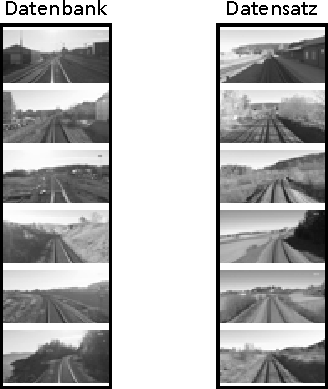
\includegraphics[width=0.4\textwidth]{../Bilder/Bildvektoren.pdf}
	\caption[Bildvektoren für den SequenceSLAM]{Beispielhafter Ausschnitt der beiden Vektoren für den SequenceSLAM. Links ist der Datenbank-Vektor, rechts der danach aufgenommene Vergleichsdatensatz. Die Bilder sind aus dem sogenannten Nordland-Datensatz (Näheres in \autoref{kap:dyn_Versuch})}
	\label{img:vec_ex}
\end{figure}
\subsubsection{Präprozessierung des Bildes}
Um die Lokalisierungsergebnisse und die Rechenergebnisse zu verbessern, werden die verwendeten Bilder aus der Datenbank, sowie die Vergleichsbilder vorverarbeitet. Hierbei werden zunächst Farbbilder in Intensitätsbilder umgewandelt. Da für die Umsetzung des Programms die kostenlos verfügbare Bildverarbeitungsbibliothek \glqq openCV\grqq verwendet wurde, wurde das standardmäßig implementierte Luminanzverfahren für die Umwandlung der Farbwerte verwendet. Hierbei werden die verschiedenen Farbkanäle nach folgender Formel gewichtet:
\begin{equation}
D(x,y)=0{,}299*R+0{,}587*G+0{,}114*B
\end{equation}

Für den Algorithmus ist das Umwandlungsverfahren jedoch nicht relevant. Es gilt nur zu beachten, dass sowohl bei den Referenzbildern der Datenbank, als auch bei den Vergleichsbildern aus dem zweiten Datensatz die gleiche Methode verwendet wird, um die resultierenden Ähnlichkeitswerte nicht zu verfälschen.

Anschließend wird das Bild auf eine Größe von 64x32 Pixeln skaliert. Dieser Wert wurde von Milford und Wyeth in ihrer ursprünglichen Veröffentlichung verwendet. In weiteren Studien wurde zudem gezeigt, dass höhere Auflösungen keine nennenswerten Verbesserungen der Ergebnisse zur Folge hatten \cite{milford2013vision}. Im Gegenteil konnten sogar mit einer Auflösung von nur 32 Bildpixeln noch beeindruckend gute Ergebnisse erzielt werden. Aufgrund der sehr geringen Bildauflösung wird die Rechenzeit für die Berechnung der absoluten Summe der Grauwertdifferenzen extrem verringert. Zudem ist selbst bei großen Datenbanken der Speicherbedarf sehr gering.

Der letzte Schritt ist eine Patch-Normalisierung des Bildes. Dafür wird das Bild in kleinere Bereiche, sogenannte Patches, unterteilt. Jeder Patch wird nun anhand folgender Formel normalisiert: 
\begin{equation}
D_{i,n}=c_1*(D_i-c_2)
\end{equation}
Hierbei gilt: 
\begin{equation*}
c_1=\frac{255}{D_{max}-D_{min}}
\end{equation*}
\begin{equation*}
c_2=D_{min}
\end{equation*}
Dieser Rechenschritt erhöht den Kontrast des Bildes und ermöglicht dadurch eine Zuordnung von zwei Bildern, selbst wenn diese fast gar keine Ähnlichkeit mehr besitzen. Zudem wirkt die Normalisierung wie ein Kantenfilter, wodurch die gerade aufgenommene Szenerie einzigartiger wird.

Das so gewonnene Bild wird anschließend wieder für die weitere Nutzung in seinem zugehörigem Vektor gespeichert. Das Ergebnis der Präprozessierung ist in folgender Abbildung anhand eines Beispiels nochmals dargestellt.
%Abbildung von Bild vorher und Bild nachher einfügen
\begin{figure}[h.t]
	\centering
%	\def\svgwidth{0.3\textwidth}
	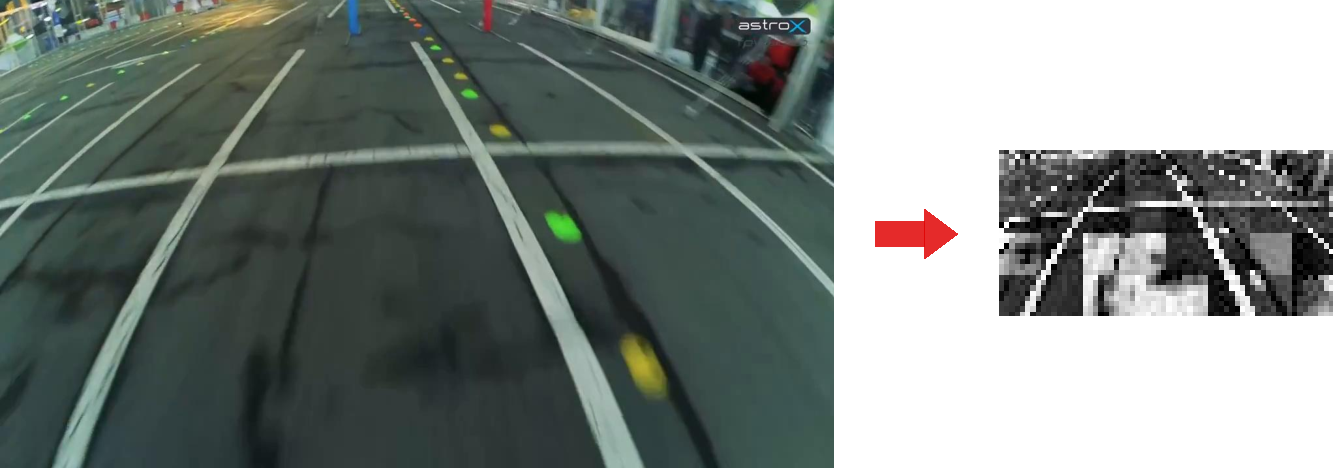
\includegraphics[width=0.85\textwidth]{../Bilder/Preprocessing_result.pdf}
	\caption[Präprozessierung des Bildes]{Präprozessierung des Bildes für den SequenceSLAM. Das Bild stammt aus einem drone-racing Video. Die Größenrelationen sind für die Visualisierung zueinander verschoben. Quelle: \url{www.youtube.com/watch?v=EcLk_uZe33w} }
	\label{img:Prepro}
\end{figure}
\subsubsection{Lokalisierung der Datensätze}
Nach der Präprozessierung der Bilder wird die Ähnlichkeit von jedem Bild aus dem Vergleichsvektor mit jedem Bild aus dem Referenzvektor bestimmt. Dies geschieht mithilfe der Summe der absoluten Grauwertdifferenzen. 
\begin{equation}
SAD=\frac{1}{N}\sum_{x=0}^{W-1}\sum_{y=0}^{H-1}D_{Ref}(x,y)-D_{Match}(x, y)
\end{equation}
$W$ und $H$ sind die Weite und die Höhe des Bildes in Pixeln. Bildet man das Produkt aus diesen beiden Größen, erhält man die Anzahl der Pixel $N$. $D$ ist der Grauwert an der Stelle $(x, y)$. 

Außer dieser Formel wurden keine weiterführenden Filteroperationen für die Ähnlichkeitsbestimmung verwendet. Die Art des Vergleichs ist jedoch laut Milford nicht relevant für den Algorithmus. Wichtig ist nur, dass ein numerischer Wert bestimmt wird, der die Ähnlichkeit zwischen den beiden Bildern beschreibt \cite{milford2012seqslam}. Die Gründe hierfür werden später nochmals beschrieben.

Anschließend wird jedes einzelne Ergebnis in eine Matrix eingetragen. Der Datenbankvektor wird in die Matrixreihen übertragen, während der Vergleichsvektor die Matrixspalten definiert. Das Ergebnis ist eine Differenzenmatrix, gefüllt mit numerischen Ähnlichkeitswerten. Diese wird im Folgenden zur besseren Visualisierung als Grauwertbild dargestellt.

\begin{figure}[!h]
	\centering
%	\def\svgwidth{0.3\textwidth}
%gestrichelte Linien Bilder --> Matrix (vertical alignment shift+strg+a)
	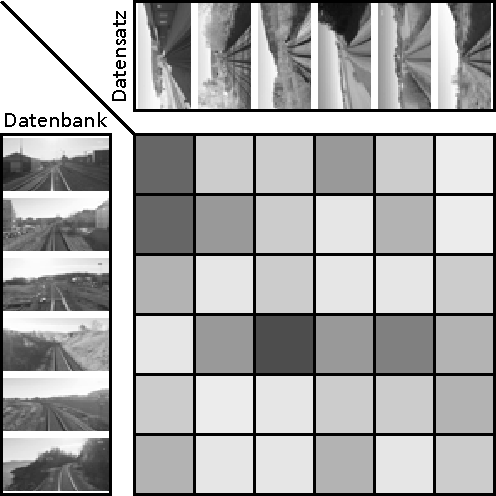
\includegraphics[width=0.6\textwidth]{../Bilder/Differenzenmatrix.pdf}
	\caption[Schematische Darstellung der Differenzenmatrix]{Schematische Darstellung der Differenzenmatrix aus den vorher gezeigten Datenvektoren. Je dunkler das Rasterfeld, desto ähnlicher sind sich die Bilder und desto wahrscheinlicher ein gefundener Match}
	\label{img:dif_Mat}
\end{figure}

Ab hier könnte bereits die Lokalisierung gestartet werden. Da jedoch zwischen zwei verschiedenen Aufnahmen Unterschiede auftreten können, wurde von Milford noch ein Zwischenschritt eingefügt, um trotzdem die ähnlichsten Bilder zu finden. Dabei handelt es sich um ein Verfahren zur lokalen Kontrastverstärkung. Jedes Matrixelement wird dabei mit seinen direkten Nachbarn aus der gleichen Spalte verglichen und mithilfe des Mittelwerts $\overline{D}_i$ und der Standardabweichung $\sigma_i$ normalisiert (siehe \autoref{eqn:Kont_Norm}). Die so ermittelten Werte werden anschließend positionsgetreu in eine neue Matrix geschrieben. 

\begin{figure}[h!]
	\centering
%	\def\svgwidth{0.3\textwidth}
	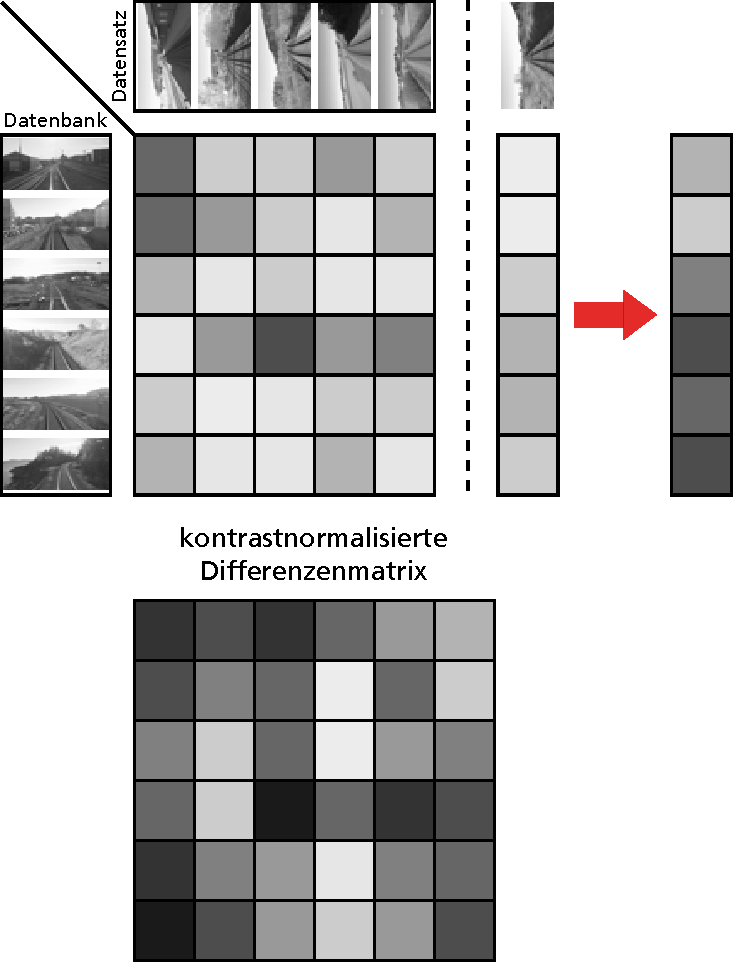
\includegraphics[width=0.8\textwidth]{../Bilder/Kontrastnormalisierung.pdf}
	\caption[Darstellung der Kontrastnormalisierung]{Kontrastnormalisierung der Ergebnismatrix. Hier ist ein beispielhafter Ausschnitt dargestellt, wie er in der Differenzenmatrix vorkommen könnte. Jede Spalte der Matrix wird nun einzeln kontrastnormalisiert und anschließend wieder positionsgetreu in die neue Matrix eingetragen.}
	\label{img:Kon_Norm}
\end{figure}

%Bild mit Vektor aus Matrix einfügen
\begin{equation}
D_i=\frac{\overline{D}_i - D_i}{\sigma_i}
\label{eqn:Kont_Norm}
\end{equation}

Abschließend findet die eigentliche Lokalisierung statt. Wie bereits erwähnt wird hierfür nach einer passenden Sequenz in der Datenbank gesucht. Da die Bilder chronologisch und in den gleichen Abständen in den Vektoren gespeichert wurden, bedeutet das, dass die ähnlichsten Orte entlang einer Geraden mit dem Steigungswinkel -$45^{\circ}$ in der Matrix liegen müssen. Bei den Aufnahmen konnten jedoch Abweichungen in der Fahrgeschwindigkeit auftreten, weshalb noch weitere Geraden mit anderen Steigungen verwendet wurden. 

%Bild mit Gerade in Differenzenmatrix
\begin{figure}[h!]
	\centering
	%linke Schrift quer
%	\def\svgwidth{0.3\textwidth}
	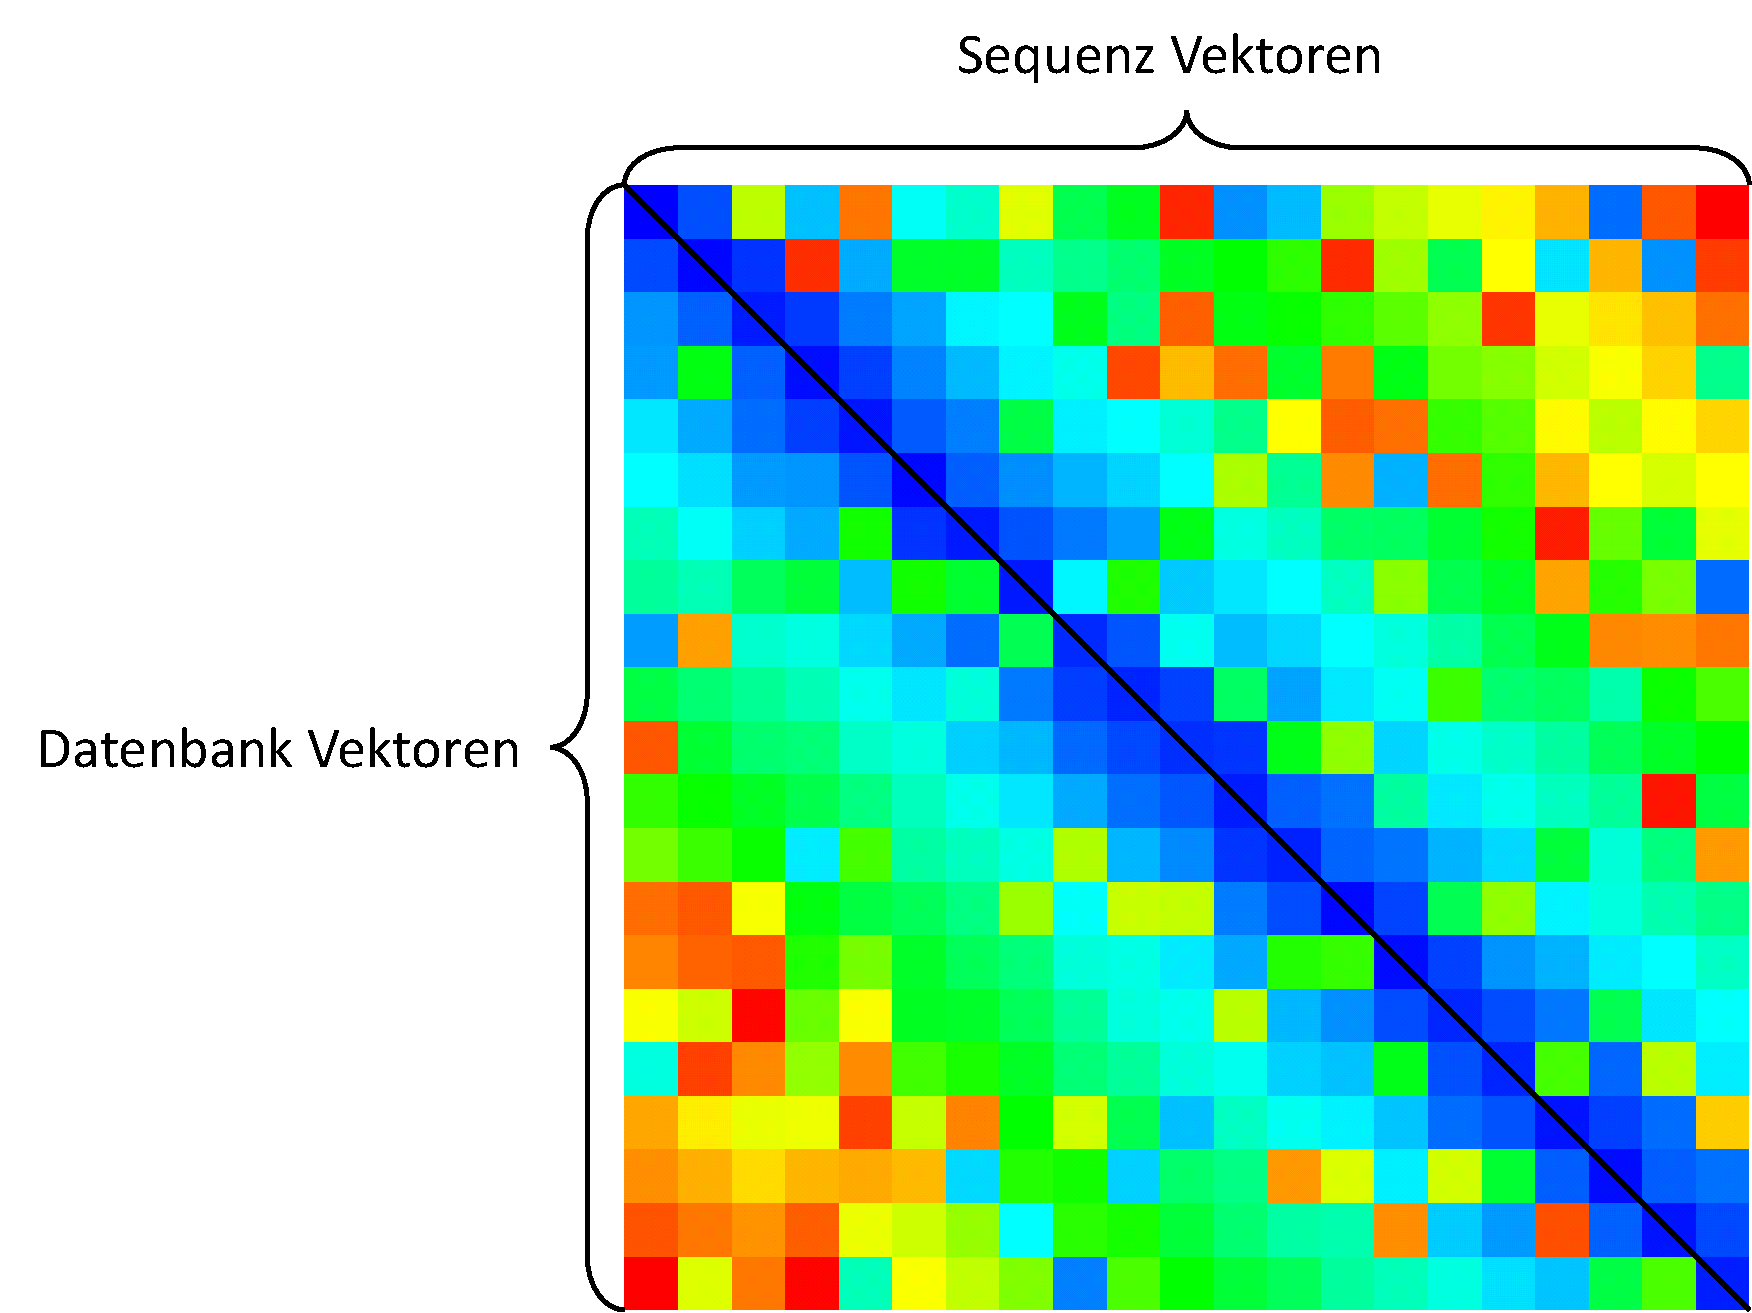
\includegraphics[width=0.7\textwidth]{../Bilder/Differenzenmatrix_mit_Gerade.pdf}
	\caption[Schematische Darstellung der Sequenzfindung]{Schematische Darstellung der Sequenzfindung. Die Differenzenmatrix wird hier in Falschfarben dargestellt (blau entspricht einer sehr hohen Ähnlichkeit, rot einer sehr geringen). Die Diagonale ist hierbei die beste Sequenz.}
	\label{img:Diff_Mat_Gerade}
\end{figure}

Für das Matching werden die Geradengleichungen definiert und diskretisiert, sodass die x- und y-Werte der Geraden den Indizes der Matrix entsprechen. Anschließend wird der Startpunkt der Geraden nach und nach auf jeden Differenzenwert in der Matrix gelegt. Die Gerade, entlang derer der geringste Wert auftritt, wird als Resultat für den aktuellen Wert an dieser Position gespeichert. Für jede Spalte, also jeden Ort im Vergleichsvektor, werden so Vektoren mit Ergebniswerten erstellt.

Da vorher die höchste Ähnlichkeit zwischen zwei Werten als $0$ definiert wurde, muss auch das aufaddierte Ergebnis der korrekten Sequenz möglichst gering sein. Aus diesem Grund wird in jedem Ergebnisvektor der Minimalwert gesucht. Der gefundene Datenbankindex beschreibt den Ort,  an dem sich das Fahrzeug momentan wahrscheinlich befindet und wird als Ergebnis der Lokalisierung ausgegeben.

Um jedoch zu verhindern, dass ein falsches Lokalisierungsergebnis ausgegeben wird, wird dieses vorher noch überprüft. Dafür wird das zweitbeste Resultat aus dem Ergebnisvektor gesucht, wobei die Werte in der direkten Umgebung des besten Matches nicht berücksichtigt werden. Anschließend wird der beste Wert durch den zweitbesten dividiert. Das Resultat ist eine Faktor zwischen null und eins, der die Einzigartigkeit der aktuellen Lokalisierung angibt. Sollte es außer dem besten Match noch ein ähnlich gutes Ergebnis geben, geht der Wert gegen 1. Daher bedeutet ein kleiner Wert, dass die Lokalisierung mit einer höheren Wahrscheinlichkeit korrekt ist. Über einen Schwellwert können anschließend die falschen oder unsicheren Ergebnisse aussortiert werden.
\newpage
\subsection{Stärken und Schwächen}
%Tabelle einfügen und danach im Text genauer beschreiben? Ohne einleitende Worte?
\begin{table}[!htp]
\fontfamily{pfr}\selectfont
\renewcommand{\tabularxcolumn}[1]{m{#1}} 
\captionabove{Auflistung der Stärken und Schwächen des SequenceSLAM Algorithmus}
\label{tab:SeqSLAM_Pro_Con}
\centering
	\begin{tabularx}{1.0\textwidth}[t]{CC}
	%\toprule
	\rowcolor[gray]{.85}\textbf{Stärken}	&	\textbf{Schwächen}\tabularnewline
	\hline
	\begin{itemize}
	\item Der SequenceSLAM ist extrem robust gegenüber Helligkeitsänderungen\newline \newline
	\end{itemize}
	&
	\begin{itemize}
	\item Es handelt sich um ein rein passives Lokalisierungsverfahren, es können also keine Bewegungsinformationen anhand der Bilder ermittelt werden.
	\end{itemize}
	\tabularnewline
	\hline
	\begin{itemize}
	\item Das Matching-Verfahren ist aufgrund des Grauwertvergleichs und der geringen Bildauflösung relativ schnell
	\end{itemize}	
	&
	\begin{itemize}
	\item Es ist nur teilautonom, da die Route vorher einmal aufgenommen werden muss.\newline
	\end{itemize}	
	\tabularnewline
	\hline
	\begin{itemize}
	\item Der Speicherbedarf (und damit die matching-Zeit) hängt linear von der Größe der Datenbank ab und ändert sich nicht während der Laufzeit
	\end{itemize}
	&
	\begin{itemize}
	\item Der Blickwinkel und andere Kamera-einstellungen beeinflussen stark die matching-Ergebnisse\newline \newline
	\end{itemize}
	\tabularnewline
	\bottomrule
	\end{tabularx}
\end{table}	
%\newpage
In Tabelle \ref{tab:SeqSLAM_Pro_Con} sind die Stärken und die Schwächen des SequenceSLAM aufgelistet. Dabei ist vor allem die Robustheit gegenüber Helligkeitsschwankungen des Algorithmus hervorzuheben. Ein entscheidender Faktor hierfür ist das Verwenden der lokal besten Ergebnisse anstatt der global besten. Dabei wird angenommen, dass der richtige Ort auf der Route ein deutlich besseres Ergebnis als seine direkten Nachbarn liefert. Gleichzeitig werden global sehr gute Ergebnisse, die allerdings keine großen Unterschiede zu den sie umliegenden Orten aufweisen, dadurch entfernt. Dieses Verfahren ist nochmal grafisch in der nachfolgenden Abbildung dargestellt. 
%Zwei Graphen, die einen Differenzvektor als Funktion von Differenzwerten darstellen. Einmal vor der Kontrastnormalisierung, einmal danach.
\begin{figure}[h]
	\centering
%	\def\svgwidth{0.3\textwidth}
	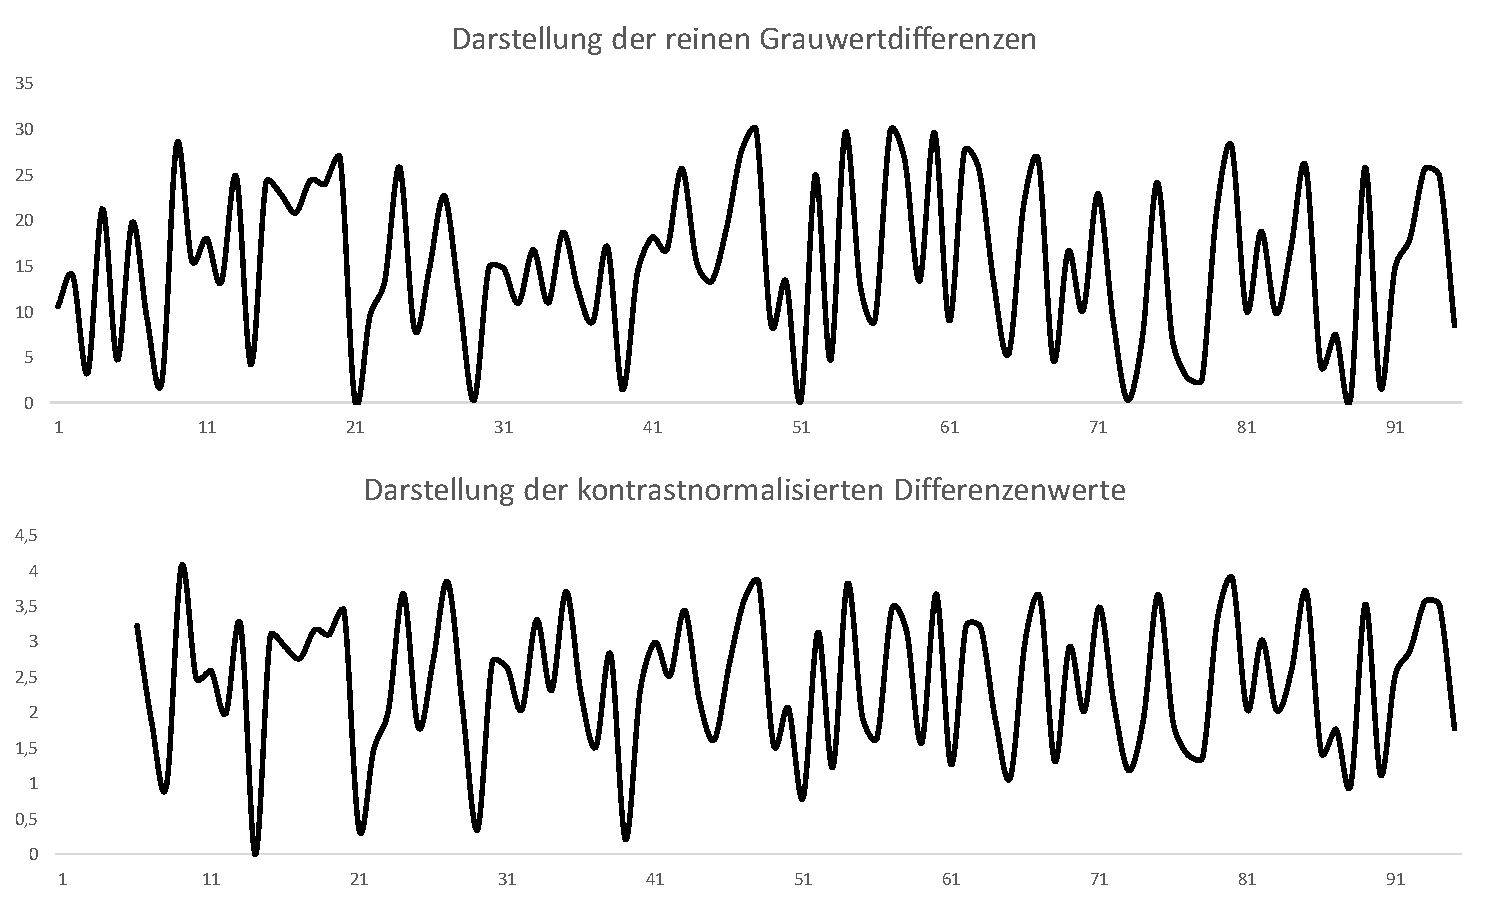
\includegraphics[width=1.0\textwidth]{../Bilder/lokale_Kontrastverstaerkung.pdf}
	\caption[Lokale Kontrastnormalisierung der Grauwertvektoren]{Darstellung der Ähnlichkeitswerte eines Differenzenvektors als Graph. Die Ähnlichkeitswerte werden hierbei auf die Bildindizes aufgetragen. Oben ist der Ähnlichkeitsvektor vor der Kontrastverstärkung dargestellt, unten danach. Der grüne Punkt ist dabei der lokal beste Match, die roten Punkte die global besten Matches.}
	\label{img:Kon_Verst}
\end{figure}

Allerdings werden durch diesen Schritt auch einige falsche Positionen als mögliche Lokalisierungen gewertet. Anhand der Sequenz können jedoch einzelne Ausreißer herausgefiltert werden (siehe Abbildung~\ref{img:Diff_Mat_Gerade}). Im optimalen Fall gibt es nur eine Sequenz von Bildern in der Differenzenmatrix. Damit dieser Fall sichergestellt werden kann, wird die Güte der Lokalisierung bestimmt mithilfe der zweitbesten Sequenz bestimmt. Ist diese zu schlecht, wird der Ort als \glqq false positive\grqq \ deklariert und verworfen.
%Bilder, die von dem Verfahren gematcht werden konnten
%Programm ohne ros-Anbindung entsprechend anpassen, dass Bilder formatiert und gespeichert werden

Die Bildunterschiede, die durch dieses Verfahren tatsächlich überwunden werden können, sind enorm. So können Orte, die einmal bei Tag und einmal bei Nacht aufgenommen wurden, tatsächlich noch korrekt einander zugeordnet werden. Ein weiterer Anwendungsfall war die Lokalisierung zu verschiedenen Jahreszeiten (siehe \cite{sunderhauf2013we}). Auch hier konnte der SequenceSLAM mit sehr guten Ergebnissen überzeugen.

Sünderhauf erwähnt in seiner Arbeit zudem, dass die Ergebnisse stark vom Blickwinkel und der perspektivischen Verzerrung der Kamera abhängen. Dadurch können Bilder, die nur um 1-2 Pixel zueinander verschoben sind, nicht mehr korrekt einander zugeordnet werden, auch wenn alle anderen Aufnahmebedingungen gleich bleiben. 

Zusätzlich wurde das Verfahren ursprünglich nicht für ein autonomes Verhalten ausgelegt. Der Algorithmus lokalisiert sich rein passiv und wird nicht als live Anwendung verwendet. Schlussendlich ist auch noch keine Methode integriert, die eine Navigation nach erfolgreicher Lokalisierung ermöglicht. 
\pagebreak
\section{Anpassungen des Algorithmus}
%Da sich dieser Teil mit dem Hauptthema meiner Arbeit beschäftigt, sollte ich hier sehr ins Detail gehen. Daher also mindestens 20 Seiten, vielleicht sogar 30?
\subsection{Vorbereitungen für die Live-Anwendung} 
Damit der Algorithmus zum autonomen Folgen einer Route verwendet werden kann, müssen zuerst die Verfahren auf eine Anwendung mit Live-Bildern angepasst werden. Hierfür wurde anstatt einer statischen Matrix, die einmal erstellt und anschließend nicht mehr verändert wird, eine dynamische Matrixerzeugung gewählt. Die Matrix wird Laufzeit des Algorithmus ständig angepasst und durch den Differenzenvektor des aktuellen Frames mit allen Datenbankbildern ergänzt.
\subsubsection{Dynamische Matrixerzeugung}
Wie beim originalen SequenceSLAM-Algorithmus muss die Datenbank einmal komplett aufgenommen werden. Im Gegensatz zum Original wird der Vergleichsdatensatz jedoch während der Laufzeit erstellt. Dafür werden die Bilder einer Kamera ausgelesen und, nachdem sie vorverarbeitet wurden, in einem Vektor mit vordefinierter Länge gespeichert. Sobald der Vektor komplett gefüllt ist, wird das älteste Bild gelöscht und dafür die neueste Aufnahme gespeichert. Dadurch entsteht nach und nach ein eindimensionaler Vektor, aus dem zusammen mit der Datenbank wieder eine Ähnlichkeitsmatrix berechnet werden kann.

Diese wird allerdings nicht bei jeder Aufnahme eines neuen Bildes komplett neu berechnet. Stattdessen wird auch hier eine feste Größe für die Matrix vorgegeben. Die Anzahl der Zeilen entspricht der Menge der Bilder in der Datenbank und die Spalten werden auf die gleiche Größe wie der Vergleichsvektor begrenzt. Sobald das Bild ausgelesen und im Vergleichsvektor gespeichert wurde, wird die Ähnlichkeit des aktuellen Bildes zu jedem einzelnen Datenbankbild bestimmt. Diese werden wiederum temporär in einem eindimensionalen Vektor gespeichert.

Anschließend wird wieder die Kontrastnormalisierung wie beim originalen Algorithmus durchgeführt. Das Ergebnis ist ein eindimensionaler, kontrastnormalisierter Differenzenvektor, der die Ähnlichkeitsinformationen des aktuellen Bildes mit den Datenbankbildern enthält. Anhand der Anzahl der vorher aufgenommenen Bilder wird der Vektor in die entsprechende Spalte der Matrix geschrieben. Dadurch wird die Rechenzeit deutlich verkürzt, da statt einer $N\times M$ Matrix nur noch ein Vektor pro Durchlauf berechnet werden muss.

\begin{figure}
	\centering
%	\def\svgwidth{0.3\textwidth}
	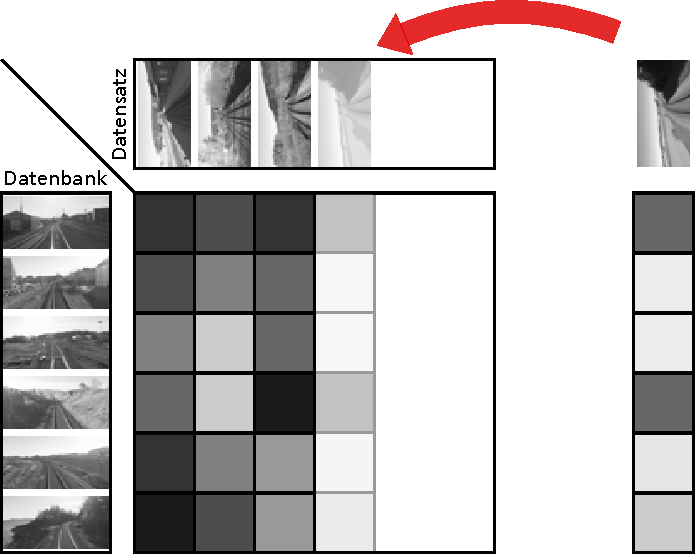
\includegraphics[width=0.7\textwidth]{../Bilder/Differenzenmatrix_live.pdf}
	\caption[Dynamische Matrixerzeugung]{Darstellung der dynamischen Matrixerzeugung. Der Vektor wird direkt nach der Bildaufnahme berechnet und normalisiert. Die Differenzenmatrix wird während der Laufzeit nach und nach erstellt.}
	\label{img:Diff_Mat_live}
\end{figure}

Wie zuvor beim Datensatzvektor auch, wird auch hier die älteste Spalte gelöscht, sobald die Anzahl der Bilder die maximale Datensatzgröße überschreitet. Damit jedoch die Lokalisierung korrekt durchgeführt werden kann, muss sichergestellt werden, dass die Bilder aus der Datenbank und aus dem Vergleichsdatensatz ungefähr an den gleichen Positionen aufgenommen werden. Sollte dies nicht der Fall sein, können die Ähnlichkeitswerte nicht mehr korrekt ermittelt werden und die Ergebnisse verschlechtern sich dementsprechend. Daher wurde über verschiedene Methoden nachgedacht, welche eine solche Synchronisation der beiden Aufnahmen ermöglicht.
%Bild einfügen von verschobenen Messpunkten und vielleicht sogar Bildern?
\subsubsection{Synchronisation der Aufnahmepunkte}
Die einfachste Methode ist hierbei das Verwenden einer zeitlichen Synchronisation zwischen Datensatz und Datenbank. Diese ist allerdings nicht immer optimal, da sich die Aufnahmepunkte immer weiter voneinander entfernen, sollten die Geschwindigkeiten nicht komplett gleich sein. Zudem besitzt sie den Nachteil, dass der Startpunkt immer gleich sein muss, da sonst die nachfolgenden Aufnahmepunkte, selbst bei gleichen Fahrgeschwindigkeiten, genau zwischen den Datenbankbildern liegen. Bei relativ hohen Aufnahmeraten und bekannten Geschwindigkeiten während der Aufnahme der Datenbank und des Datensatzes, ist die zeitliche Synchronisation jedoch trotzdem anwendbar.

Eine weitere Methode, die bereits in früheren Arbeiten zum SequenceSLAM verwendet wurde, ist das Verwenden von Odometrie-Daten. Da inzwischen jedes Fahrzeug, sowohl zu Land, als auch in der Luft, eine Sensorik zur Überwachung der Beschleunigungen und der Geschwindigkeiten besitzt, können die Positionsdaten relativ genau berechnet werden. Dafür werden zunächst die Abstände zwischen den Aufnahmepunkten der Referenzfahrt bestimmt und gespeichert. Bei der zweiten Fahrt werden ebenfalls die Abstände des Fahrzeugs zum letzten Aufnahmepunkt gemessen und, sobald dieser einen bestimmten Schwellwert überschreitet, die Aufnahme getriggert. 

Dieses Verfahren liefert zwar keine ground-truth-Daten, es ist jedoch in den meisten Fällen ausreichend, um die Aufnahmepositionen miteinander zu synchronisieren, sofern nicht korrigierbare Störfaktoren wie ein Rutschen der Räder ausgeschlossen werden können. Zudem können hierdurch im Gegensatz zur zeitlichen Synchronisation Geschwindigkeitsunterschiede während der Aufnahme ausgeglichen werden. Da jedoch keine ground-truth-Daten vorliegen, bleibt auch hier das Problem, dass der Startpunkt bei beiden Aufnahmen gleich sein muss, um ein korrektes Matching zu gewährleisten.

Die letzte Methode zur Synchronisation wäre das Verwenden von übergeordneten Lokalisierungsmethoden wie zum Beispiel das Global Positioning System (GPS). Dadurch können für jeden Aufnahmepunkt ground-truth-Daten bereitgestellt werden und somit eine perfekte Synchronisation unabhängig von den Geschwindigkeiten und dem genauen Startpunkt gewährleistet werden. Der Nachteil hierbei ist, dass der Algorithmus dann nicht in Gegenden eingesetzt werden kann, wo es keine solch übergeordnete Systeme gibt. Außerdem wäre dann in jedem Fall aufwendige, externe Sensorik notwendig, die den gesamten Aufbau unnötig kompliziert machen würde. Die vorherigen Methoden würden mit der bordeigenen Sensorik funktionieren. 

Die Vor- und Nachteile dieser Methoden sind zur besseren Visualisierung nochmals in nachfolgender Tabelle aufgelistet.
\begin{table}[!htp]
\fontfamily{pfr}\selectfont
\renewcommand{\tabularxcolumn}[1]{m{#1}} 
\captionabove{Übersichtstabelle über die Vor- und Nachteile der verschiedenen Synchronisationsarten}
\label{tab:Synchro}
\centering
	\begin{tabularx}{1.0\textwidth}[t]{C|CCC}
	%\toprule
	\rowcolor[gray]{.85}
	\textbf{Art der Synchronisation}	&	\textbf{Startplatz-unabhängig} & \textbf{Geschwindigkeits-unabhängig} & \textbf{mit bordeigener Sensorik}\tabularnewline
	zeitliche Synchronisation & \xmark & \xmark & \cmark \tabularnewline
	odmetrische Synchronisation & \xmark & \cmark & \cmark \tabularnewline
	externe Synchronisation & \cmark & \cmark & \xmark
	\end{tabularx}
\end{table}

Aufgrund der aufgezeigten Stärken und Schwächen wird empfohlen, eine odometrische Synchronisation für eine reale Anwendung zu verwenden. In Simulationsumgebungen, in denen alle Parameter bekannt sind und die Experimentierbedingungen dementsprechend reproduziert werden können, reicht auch eine zeitliche Synchronisation der Aufnahmepunkte. 

Von einer externen Synchronisation wird komplett abgeraten, da die benötigte Sensorik und deren Einbindung extrem hohen Aufwand und zusätzliche Kosten bedeuten würde. Zudem werden optische Navigationsverfahren gerade in Gegenden benötigt, wo solch eine externe Lokalisierung nicht möglich ist. 
%\subsubsection{Variable Aufnahmefrequenz}
%Die soeben vorgestellten Verfahren zur Steuerung der Bildaufnahme können die Genauigkeit des Matchings bei Live-Aufnahmen bereits enorm erhöhen. Wenn allerdings einmal ein Fehler bei der Aufnahmesteuerung auftritt beeinflusst das alle weiteren Aufnahmen. Dadurch kann der Fehler immer größer werden, bis schließlich kein gutes matching-Ergebnis gefunden werden kann. 
%
%Da der Algorithmus bis zu dem Punkt an dem er sich nicht mehr lokalisieren konnte immer der vorgegebnen Route gefolgt sein muss, muss sich der nächste Aufnahmepunkt in der Nähe der aktuellen Position befinden. Im optimalen Fall liegt er genau auf der momentanen Fahrbahn des Roboters. In diesem Fall kann der Fehler, der bei der Aufnahmensteuerung geschehen ist, behoben werden. Dafür wird ab dem Punkt, an dem die Lokalisierung fehlgeschlagen ist, die Aufnahmefrequenz auf den maximal möglichen Wert erhöht. 
%
%Die neuen Bilder werden allerdings nicht als neues Bild in den Live-Vektor eingetragen. Dies würde nur die Berechnung einer Matching-Sequenz behindern. Stattdessen wird das letzte eingetragene Bild, das nicht korrekt lokalisiert wurde von dem aktuellen überschrieben. Anschließend wird wieder der Differenzenvektor berechnet und an die entsprechende Stelle in die Matrix eingetragen. 
%
%Auf diese Weise wird weiterhin Bild um Bild aufgenommen, bis eine der Aufnahmen eine matchbare Sequenz ermöglicht. Ab diesem Punkt kann sich der Algorithmus wieder korrekt lokalisieren und die Route des Roboters wieder korrigieren. 
\subsection{Dynamische Ermittlung der Sequenzlänge}
Wie bereits erwähnt, dokumentierten Milford und Wyeth in ihrer Arbeit, dass mithilfe des SequenceSLAM eine Matching"=Quote von ca. $33\%$ erreicht werden konnte, ohne dass dabei falsche Lokalisierungen stattfanden. Obwohl dieses Ergebnis in Hinblick auf die großen Unterschiede zwischen den Aufnahmen erstaunlich war, wird für eine erfolgreiche Navigation eine deutlich höhere Lokalisierungsrate benötigt.

Die entscheidenden Parameter des SequenceSLAM, die die Lokalisierungsergebnisse  am meisten beeinflussen, sind hierbei die Länge der verwendeten Sequenz und das Vergleichsverfahren. Hierzu haben bereits Sünderhauf et al. in ihrer Arbeit ausführliche Experimente mit verschiedenen Parametereinstellungen durchgeführt \cite{sunderhauf2013we}. 

Dabei fanden sie heraus, dass eine längere Sequenz auch eine höhere Lokalisierungsrate bedeutete. Dafür wurden die Lokalisierungen ungenauer, wodurch auch einige falsche Ergebnisse gefunden wurden. Zudem wurden die Ergebnisse ab einer Länge von mehr als 100 Bildern wieder schlechter, da nun die Sequenzen zu unspezifisch waren. Ein weiterer Negativpunkt war die deutlich erhöhte Rechenzeit im Vergleich zu den kleineren Sequenzen. 

Um die Vorteile beider Sequenzlängen zu kombinieren, wurde eine dynamische Anpassung dieser Größe während der Laufzeit implementiert. Jedes Bild wird dabei zuerst mithilfe der Standardsequenzlänge überprüft. Sollte das Ergebnis unter dem gewählten Schwellwert sein, wird es als wahr gewertet und die Position in der Datenbank ausgegeben. Ist es dahingegen zu schlecht, werden im nächsten Schritt doppelt so viele Bilder in die Sequenz geladen. Anschließend wird wieder gematcht und das Ergebnis ausgewertet. Sollte die aktuelle Lokalisierung wieder zu schlecht sein, wird der Vorgang solange wiederholt, bis die maximale Sequenzlänge von 100 Bildern erreicht wurde, oder keine weiteren Datensatzbilder im Vektor mehr gespeichert sind.

Wenn ab diesem Punkt immer noch kein zufriedenstellendes Ergebnis ermittelt werden konnte, wird das aktuelle Bild als \glqq nicht lokalisierbar\grqq{ }deklariert und das nächste Bild in den Vergleichsvektor geladen. Auf diese Weise wird jeder Ort so präzise wie möglich lokalisiert, während die Laufzeit nicht allzu sehr vergrößert wird.

Um zu überprüfen, ob dieses Verfahren eine Verbesserung zum originalen SequenceSLAM darstellte, wurden anschließend Versuche durchgeführt. Dabei waren folgende Faktoren entscheidend:
\begin{itemize}
\item Können mehr Orte korrekt lokalisiert werden?
\item Werden mehr \glqq false positives\grqq~lokalisiert?
\item Erhöht sich die Laufzeit des Algorithmus?
\end{itemize}
\subsubsection{Versuchsbedingungen}\label{kap:dyn_Versuch}
Zum Testen wurde der sogenannte "Nordland-Datensatz" verwendet. Dabei handelt es sich um die Aufnahme einer 728 km langen Bahnstrecke aus der Perspektive des Zugfahrers. Sie wurde insgesamt viermal aufgenommen, einmal zu jeder Jahreszeit. Die Aufnahme wurde im Rahmen der TV-Dokumentation "Norlandsbanen - Minutt for Minutt" vom norwegischen Fernsehsender NRK aufgenommen und ist online auf der Seite \url{http://nrkbeta.no/2013/01/15/nordlandsbanen-minute-by-minute-season-by-season/} als \glqq Common Creative license\grqq~erhältlich. 

Sünderhauf et al. verwendeten bereits diesen Datensatz, um die Robustheit des Algorithmus gegenüber jahreszeitlichen Schwankungen zu bewerten. Dafür hat er einen halbstündigen Ausschnitt aus jeder der vier Aufnahmen ausgeschnitten und mithilfe von ebenso verfügbaren GPS-Daten synchronisiert. Auf diese Weise erhielt er vier Datenbanken, die an jedem Index den genau gleichen Ort zu unterschiedlichen Jahreszeiten zeigte. Diese bereits synchronisierten und vorverarbeiteten Bilder wurden von ihm für weitere Tests ebenfalls online hochgeladen (\url{https://svn.openslam.org/data/svn/openseqslam/trunk/datasets/}).

Wie bereits erwähnt eigneten sich diese Datensätze, um die Robustheit gegenüber jahreszeitlichen, aber auch gegen Helligkeitsschwankungen zu testen. So sind die Bilder im Winter aufgrund des Schnees deutlich heller, als zum Beispiel im Herbst. Allgemein sind die gleichen Orte in den vier Datenbanken teilweise so unterschiedlich, dass ein reiner Grauwertvergleich beinahe keine Ähnlichkeit mehr ermitteln kann. 
\begin{figure}[ht]
	\centering
%	\def\svgwidth{0.3\textwidth}
	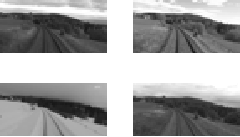
\includegraphics[width=0.65\textwidth]{../Bilder/Nordland_Datensatz.pdf}
	\caption[Beispiel Bilder aus dem Nordland-Datensatz]{einige Beispielbilder aus dem Nordland-Datensatz. Jedes Bild zeigt den gleichen Ort zu unterschiedlichen Jahreszeiten: Oben links im Herbst, Oben rechts im Frühling, unten links im Winter und unten rechts im Sommer.}
	\label{img:Nordland}
\end{figure}

Für den Test wurden jeweils 350 Bilder aus den Datensätzen \glqq Sommer\grqq{ }und \glqq Winter\grqq{ }verwendet. Der Abstand zwischen den einzelnen Bildern lag bei 100 Datenbankbildern. Der Algorithmus wurde dabei mit c++ geschrieben und auf einem 32 Bit SUSE Enterprise-Linux-System angewendet. Für die Tests war bereits die live-Berechnung der Differenzenmatrix implementiert worden. Der erste Durchlauf fand ohne die dynamische Anpassung der Sequenzlänge statt, der zweite Versuch mit ihr. Ansonsten wurden keine Änderungen am Algorithmus vorgenommen. Gemessen wurde neben der Laufzeit auch, wie viele Bilder lokalisiert werden konnten und wie viele nicht. Bei den lokalisierten Orten wurde zudem noch zwischen korrekten und falschen Ergebnissen unterschieden. Ein Ergebnis galt als falsch, wenn der gefundene Datenbankindex mehr als eine Stelle zum gesuchten Index verschoben war. 
\subsubsection{Versuchsergebnisse}
\begin{table}[!h.t]
\fontfamily{pfr}\selectfont
\renewcommand{\tabularxcolumn}[1]{m{#1}} 
\newcolumntype{A}[1] {>{\centering}m{#1}}
\captionabove{Matchingergebnisse mit und ohne dynamischer Sequenzlänge}
\label{tab:dyn_Seq_Len}
\centering
	\begin{tabularx}{1.0\textwidth}[t]{CA{7 cm}C}
	%\toprule
	\rowcolor[gray]{.85}
		&	\textbf{korrekte Matches/ inkorrekte Matches} & \textbf{Durchschnittliche Laufzeit pro Bild} \tabularnewline
	\textbf{Durchlauf ohne dynamische Sequenzanpassung}	&	$137/ 0$	&	$15{,}7 ms$ \tabularnewline
	\textbf{Durchlauf mit dynamischer Sequenzanpassung}	&	$271/ 0$	&	$23{,}7 ms$ \tabularnewline
	\end{tabularx}
\end{table}

Beim ersten Durchlauf ohne Anpassung der Sequenzlänge wurde imemr über eine Sequenz von 10 Bilder gematcht. Dabei konnten insgesamt 137 Bilder aus dem Winter-Datensatz dem Sommer-Datensatz korrekt zugeordnet werden, wobei keine falschen Lokalisierungen auftraten. Insgesamt wurden somit 213 Datenbankbilder nicht lokalisiert. Damit lag die Matching-Quote bei $39{,}1 \%$, was ungefähr den Ergebnissen aus dem originalen SequenzSLAM-Paper entsprach. Die Gesamtlaufzeit vom Starten des Algorithmus bis zum Überprüfen des letzten Bildes und der Ausgabe des Ergebnisses lag bei ca. $5{,}5$ Sekunden.

Im Gegensatz dazu wurden beim zweiten Durchlauf mit der dynamischen Sequenzanpassung 271 Bilder korrekt lokalisiert, wobei ebenfalls keine falschen Lokalisierungen vorkamen. 79 Bilder konnten dementsprechend nicht zugeordnet werden. Somit lag die Matching-Quote bei $77{,}4 \%$. Die Gesamtlaufzeit des Algorithmus wurde hier mit $8{,}3$ Sekunden gemessen.

Anhand des durchgeführten Experiments kann gezeigt werden, dass die dynamische Sequenzanpassung die Lokalisierungsergebnisse deutlich verbessert. Es können beinahe doppelt so viele Matches gefunden werden, wobei die Rate an falschen Matches nicht verschlechtert wird. Allerdings wurde die Laufzeit um ca. 3 Sekunden erhöht, was beinahe $60 \%$ mehr  Laufzeit entsprach. Pro gematchtem Bild war diese trotzdem noch sehr gut im Vergleich zu anderen Algorithmen. 
\subsection{Sequenzbildung}
Ein weiterer Aspekt, der die Live-Anwendung des Algorithmus behinderte, war die mathematische Berechnung der matching-Geraden. Diese hatten ihren Ausgangspunkt immer die Anzahl Bilder einer Sequenz in der Vergangenheit. Das bedeutet, dass nicht das aktuelle Bild, sondern ein schon längst vergangenes lokalisiert wird. 
\begin{equation}
\vec{g}_{i}=(n+v*i)+(m-10+i)*D_{max}
\end{equation}
Dadurch können jedoch ungenaue Ergebnisse entstehen, was anhand folgender Abbildung verdeutlicht werden soll.
%Abbildung mit Matrix und Geraden?
Um solchen Fehlern vorzubeugen, wurde der Startpunkt, ähnlich wie in \cite{wang2015improved} auf das aktuelle Bild gelegt und die Gerade von dort in die Vergangenheit gebildet. Dadurch ergibt sich folgende Formel für die jeweiligen Geraden.
\begin{equation}
\vec{g}_{i}=(n-v*i)+(m-i)*D_{max}
\end{equation}
Hierbei ist $\vec{g}$ der Vektor mit den Indizes der jeweiligen Bilder entlang der Geraden, $m$ das aktuelle Sequenzbild und $n$ das aktuell gematchte Datenbankbild. Um verschiedene Geraden mit verschiedenen Geschwindigkeiten zu ermitteln, wird diese noch als Steigungsfaktor in die Berechnung mit einbezogen. $D_{max}$ beschreibt die Anzahl der Bilder in der Sequenz. Auf diese Weise wird ein Vektor mit den Indizes der Differenzenwerte in der Matrix berechnet. Da diese jedoch immer natürliche Zahlen sein müssen, werden die ermittelten Ergebnisse noch zur $0$ hin gerundet. Zudem findet eine Bereichsüberprüfung statt, damit nicht auf Speicher außerhalb der Matrix zugegriffen wird.

Der nächste Schritt ist dann, wie bereits zuvor, die Addition der einzelnen Werte und das Ermitteln des besten Ergebnisses. Werden die Aufnahmepunkte der beiden Fahrten zudem perfekt synchronisiert, liegt der beste Match genau auf einer Geraden mit der Steigung $-1$. Dadurch kann dann die Geschwindigkeit als Steigung für die Berechnung weggelassen werden. Da dies allerdings nicht sichergestellt werden kann und die zusätzliche Rechenzeit keinen großen Einfluss auf die Gesamtrechenzeit besitzt, wurde dieser Faktor trotzdem beibehalten. 
\subsection{Umgang mit sich selbst wiederholenden Routen}
%Kapitel neu schreiben und Dynamische Ermittlung der Sequenzlänge anpassen.
Je nachdem wie die Route aufgebaut ist, kann es passieren, dass einzelne Streckenabschnitte mehrmals passiert werden müssen. Dementsprechend wird dieser Abschnitt auch mehrfach aufgenommen und für eine Karte oder eine Datenbank gespeichert. 

%Kreis schwarz, nur mittlerer Abschnitt rot.
\begin{figure}[h.t]
	\centering
%	\def\svgwidth{0.3\textwidth}
	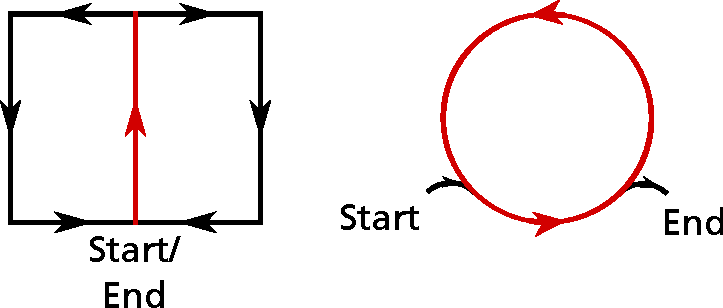
\includegraphics[width=0.5\textwidth]{../Bilder/Loop_Closure_Beispiele.pdf}
	\caption[Beispiele für Routen mit Loop Closure]{Beispielhafte Darstellung zweier Routen, bei denen Streckenabschnitte mehrfach nachgefahren werden. Beim linken Beispiel wird der mittlere Streckenabschnitt mehrfach passiert, beim rechten wird der gesamte Kreis nehrfahch umfahren, bevor das Fahrzeug beim Endpunkt ankommt.}
	\label{img:Loop_Clos_Ex}
\end{figure}
Der ursprüngliche SequenceSLAM kann mit solchen mehrfach vorkommenden Streckenabschnitten nicht umgehen. Sind zwei gleiche Orte in der Datenbank vorhanden können dementsprechend auch zwei gleich gute Ergebnisse beim Matching gefunden werden. Während eines der beiden Ergebnisse als bester Match gewertet wird, wird das andere als zweitbester Match deklariert. Die anschließende Überprüfung würde daher einen Wert nahe $1$ ergeben, wodurch die Lokalisierung nicht gewertet wird. 

Zur besseren Visualisierung wurde die Fahrt der linken Route in \autoref{img:Daten_Zeitstrahl} als Zeitstrahl dargestellt und die einzelnen Bereiche beschriftet. \glqq M\grqq{ }ist der mittlere, \glqq L\grqq{ }der linke und \glqq R\grqq{ }der rechte Streckenabschnitt. Die einzelnen Punkte markieren hierbei die Startpunkte der Geraden.

\begin{figure}[ht]
	\centering
	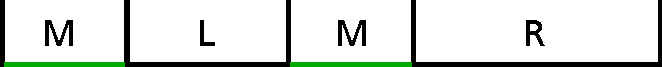
\includegraphics[width=0.6\textwidth]{../Bilder/datenbank_zeitstrahl.pdf}
	\caption[Schematische Darstellung der Datenbank]{Aufteilung der linken Route in einen Zeitstrahl. Die sich wiederholenden Bereiche sind grün markiert.}
	\label{img:Daten_Zeitstrahl}
\end{figure}
Aus diesem Grund wurden zwei Möglichkeiten erdacht, die dem Algorithmus einen Anhaltspunkt geben, wo er sich gerade in der Datenbank befindet. Bei der ersten Methode wird die Datenbank vorher bearbeitet und die mehrfach vorkommenden Bereiche speziell markiert. Beim anschließenden Matching wird dem Algorithmus mitgeteilt, wie oft er bereits den jeweiligen Abschnitt passiert hat. Nur dieser wird aus der Liste der Abschnitte für das Matching berücksichtigt. Die anderen mehrfachen Abschnitte werden nicht berücksichtigt, bis der Abschnitt komplett passiert wurde.

\begin{figure}[ht]
	\centering
	
\includegraphics[width=0.6\textwidth]{../Bilder/loop_closure_erste_methode.pdf}
	\caption[Methode 1 zur Schleifenbehandlung]{Zeitstrahl der Strecke mit nummerierter Beschriftung. Der Abschnitt, der nicht beachtet wird, wurde ausgegraut.}
	\label{img:Loop_Clos_1}
\end{figure}
Eine weitere Methode ist die Begrenzung des Suchbereichs. Hierbei werden die Matching-Geraden nur innerhalb eines bestimmten Bereichs ermittelt und ausgewertet. Der Bereich wird dabei nach und nach innerhalb der Datenbank verschoben. Alle Datenbankbilder außerhalb der Grenzen werden für das Matching nicht beachtet. 

\begin{figure}[ht]
	\centering
	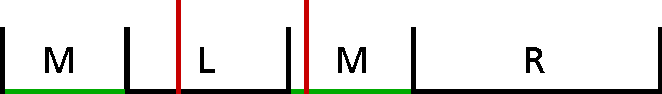
\includegraphics[width=0.6\textwidth]{../Bilder/loop_closure_zweite_methode.pdf}
	\caption[Methode 2 zur Schleifenbehandlung]{Zeitstrahl der Strecke mit rot markiertem Suchbereich.}
	\label{img:Loop_Clos_2}
\end{figure}
Für diese Arbeit wurde die zweite Methode verwendet. Dies liegt vor allem daran, dass dabei keine aufwendige Bearbeitung der Datenbank vor dem ersten Durchlauf nötig ist. Daher funktioniert der Algorithmus auch relativ schnell mit jeder beliebigen Route mit sich wiederholenden Streckenabschnitten. Zudem werden Störungen beim Zählen der bereits passierten Abschnitte vermieden. 

Die aktuellen Grenzen des Suchbereichs werden anhand der letzten bekannten Position des Roboters in der Datenbank festgelegt. Diese wird jedesmal, wenn ein Sequenzbild erfolgreich gematcht wird, aktualisiert. Aufgrund dessen, dass das Fahrzeug einer fest vorgegebenen Route folgen soll, kann die nächste Position in der Datenbank relativ genau eingegrenzt werden. Um jedoch Abweichungen von der erwarteten Position abzufangen wird dieser Bereich vergrößert. Zudem werden noch Vergleichssequenzen benötigt, um die Güte des Matchings zu berechnen. 

Der Suchbereich darf jedoch auch zu groß sein, da sonst die Vorteile der Eingrenzung wieder verloren gehen. Genaugenommen darf die Anzahl der Bilder innerhalb der Grenzen nicht größer sein als der minimale Abstand zwischen zwei sich wiederholenden Orten in der Datenbank. 
%Einfügen eines Bildes?

Der Matchingvorgang wird dabei nicht verändert. Zuerst wird das beste Ergebnis im Bereich gesucht und danach der Quotient mit dem zweitbesten Ergebnis ermittelt. Liegt dieser unter einem bestimmten Schwellwert, wird die Lokalisierung als korrekt gewertet. 

Neben der höheren Robustheit gegenüber langen Schleifenfahrten, werden aber auch andere Störeffekte eliminiert. So werden Routenabschnitte, die ähnlich aussehen wie der eigentliche Ort, an dem sich der Rover befindet, nicht mehr miteinbezogen und verfälschen so nicht mehr die Lokalisierungsergebnisse. Ein weiterer Vorteil ist die nun verringerte Rechenzeit. Anstatt über die gesamte Datenbank den korrekten Ort zu lokalisieren, ist der Abschnitt der Datenbank nun immer gleich klein. Somit kann gerade bei sehr großen Datenbanken von 1000 Bildern oder mehr die Laufzeit deutlich verringert werden.
\subsection{Schwärzen des Himmels}
Der Himmel hat einen starken Einfluss auf die Ermittlung der Ähnlichkeit zwischen den einzelnen Aufnahmen. Das Bild eines Ortes kann je nach Wetterlage stark in Helligkeit und Kontrast variieren. Das Sequenzmatching soll zwar gerade diese Störeffekte weitestgehend elminieren. Trotzdem wäre es von Vorteil, wenn der Himmel keinen so starken Einfluss mehr auf die Lokalisierungsergebnisse hat.

Dafür haben Pepperel et al. das sogenannte \glqq sky blackening\grqq\;eingeführt \cite{pepperell2013towards}. Hierbei handelt es sich um einen Prozess, der zuerst die Himmelsregion von der restlichen Umgebung separiert und anschließend komplett einschwärzt. Dadurch wird der Algorithmus noch robuster gegenüber Wetter- oder Tageszeitenschwankungen. 
\subsubsection{Bildtransformation zur Kontrasterhöhung des Himmels}
Für die Detektion des Himmels wird zunächst ein RGB-Farbbild benötigt. Anschließend wird eine Transformation angewendet, die mithilfe der drei Farbkanäle den Kontrast der Himmelsregion erhöht \cite{thurrowgood2009vision}.
\begin{equation}
C=-1{,}16*R+0{,}363*G+1{,}43*B-82,3
\end{equation}
Anhand dieser Transformation werden Bildpixel mit einem hohen Blau- und Grünanteil aufgehellt, während solche mit einem hohen Rotanteil verdunkelt werden. Da der Himmel von Natur aus einen sehr hohen blau-Anteil besitzt und im Allgemeinen auch heller als die Umgebung ist, wird er aufgehellt. Der Boden hingegen ist dunkler und besitzt höhere Rotanteile als der Himmel. Die Pixelwerte liegen dabei in einem Bereich von $-378{,}1$ bis $374{,}915$. 
%Beispielbild mit zugehörigem Histogramm einfügen

\begin{figure}[ht]
\centering
\begin{subfigure}[c]{0.49\textwidth}
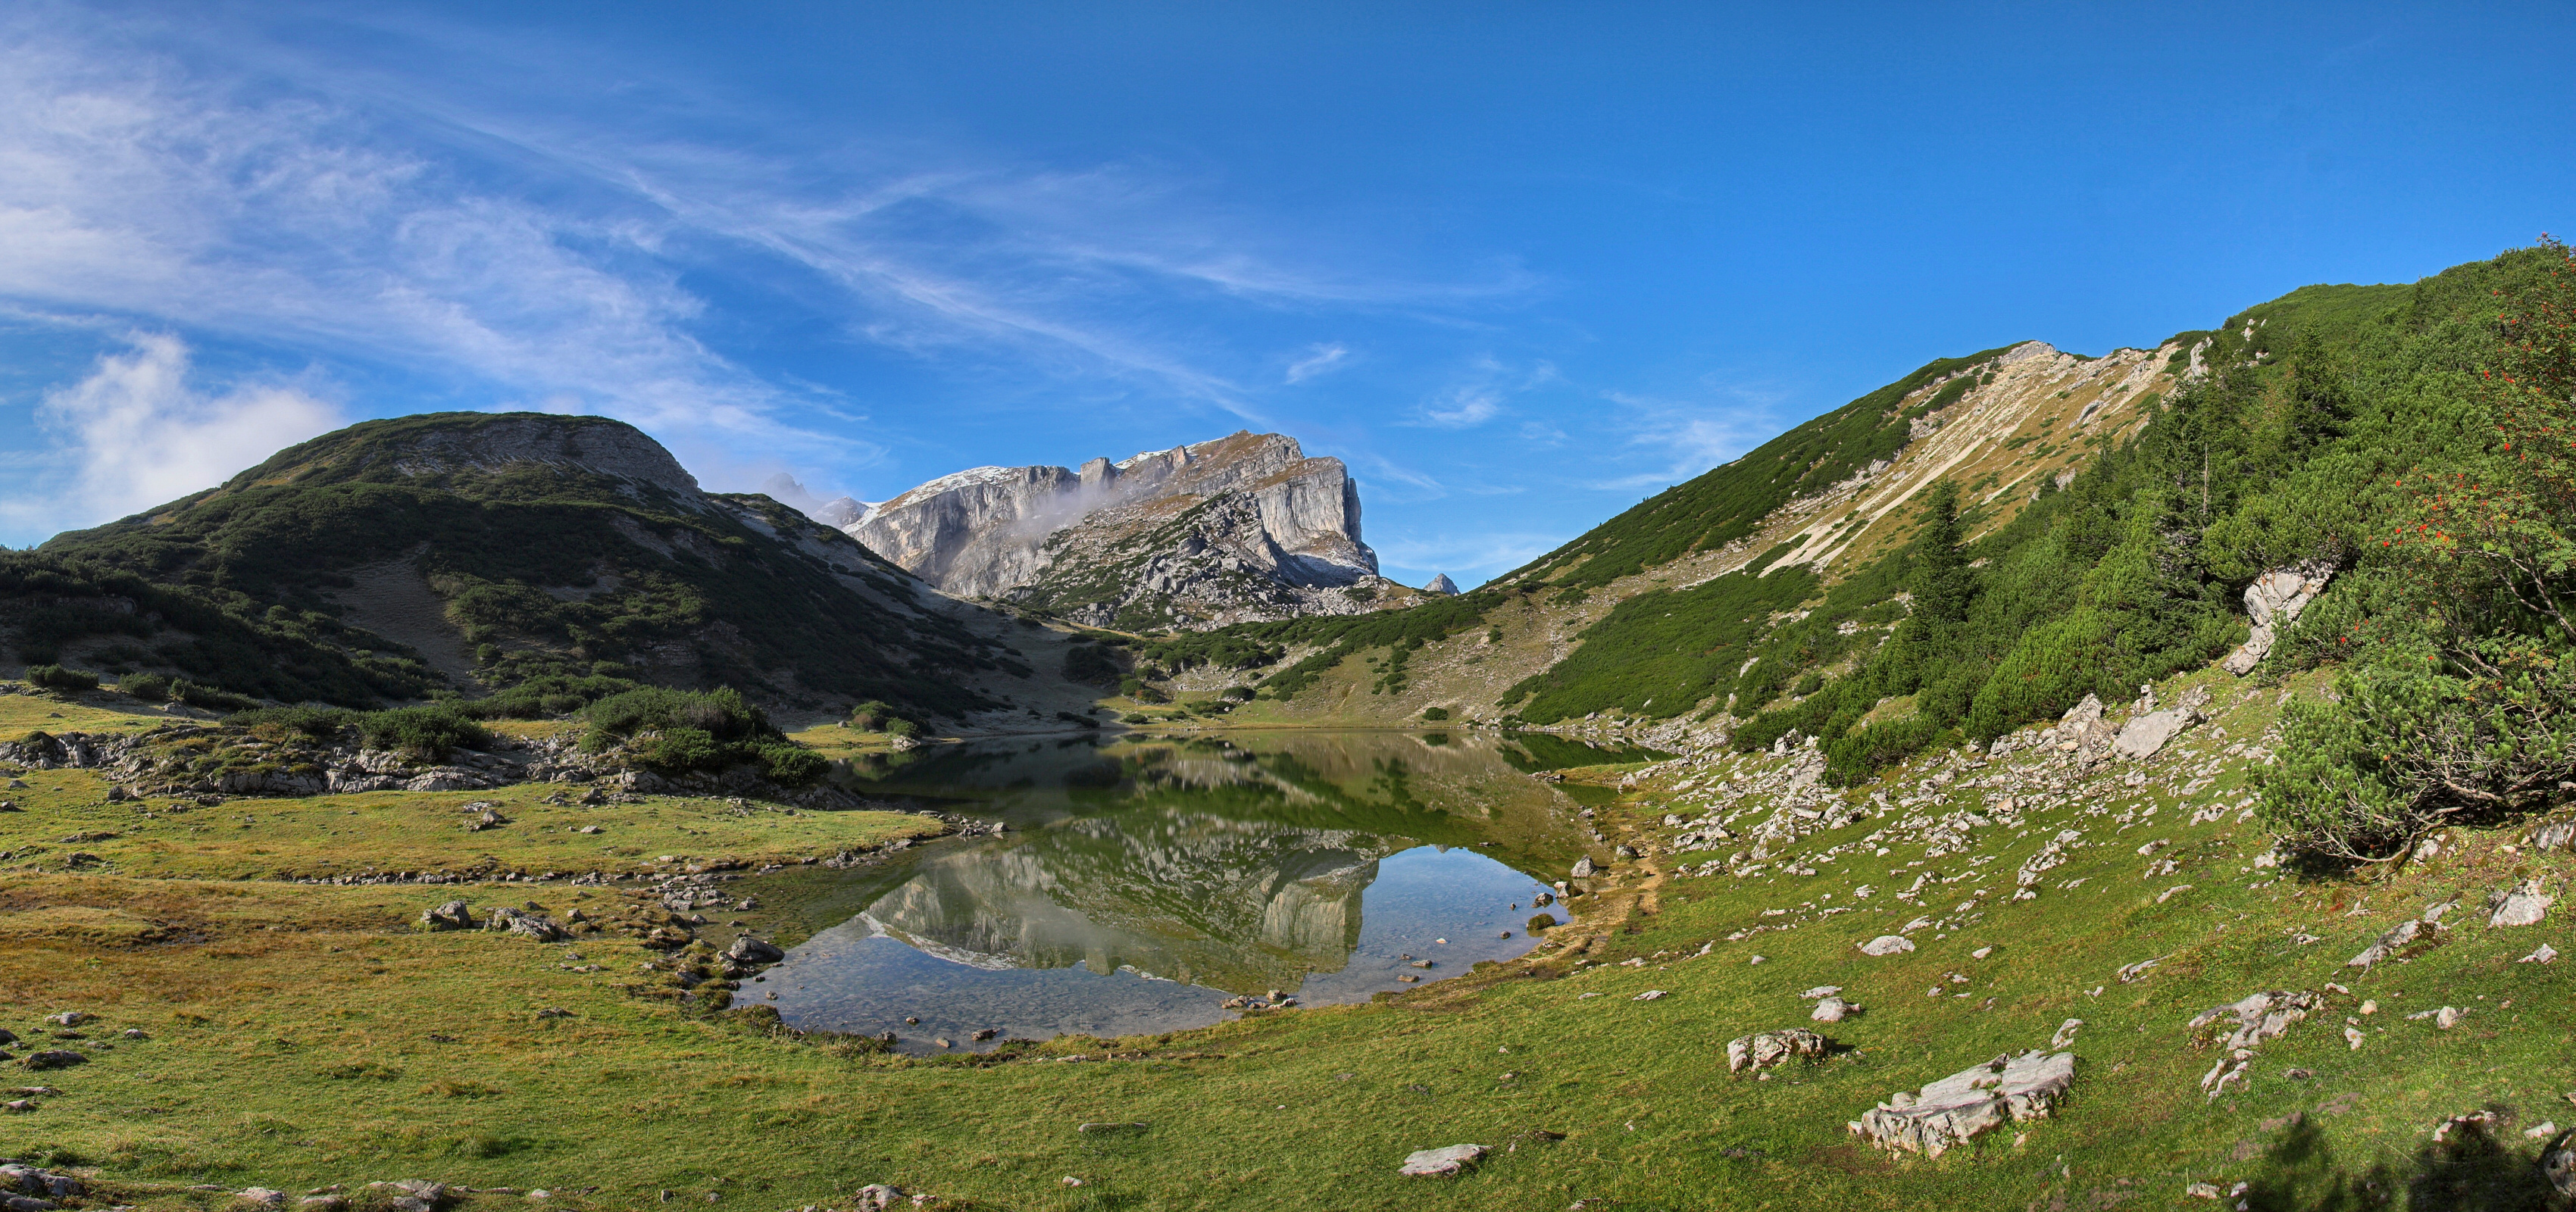
\includegraphics[width=\textwidth]{../Bilder/Zireiner_See_Rofanspitze_2006_10.jpg}
\subcaption{Originalbild}
\label{simg:Orig}
\end{subfigure}
%
\begin{subfigure}[c]{0.49\textwidth}
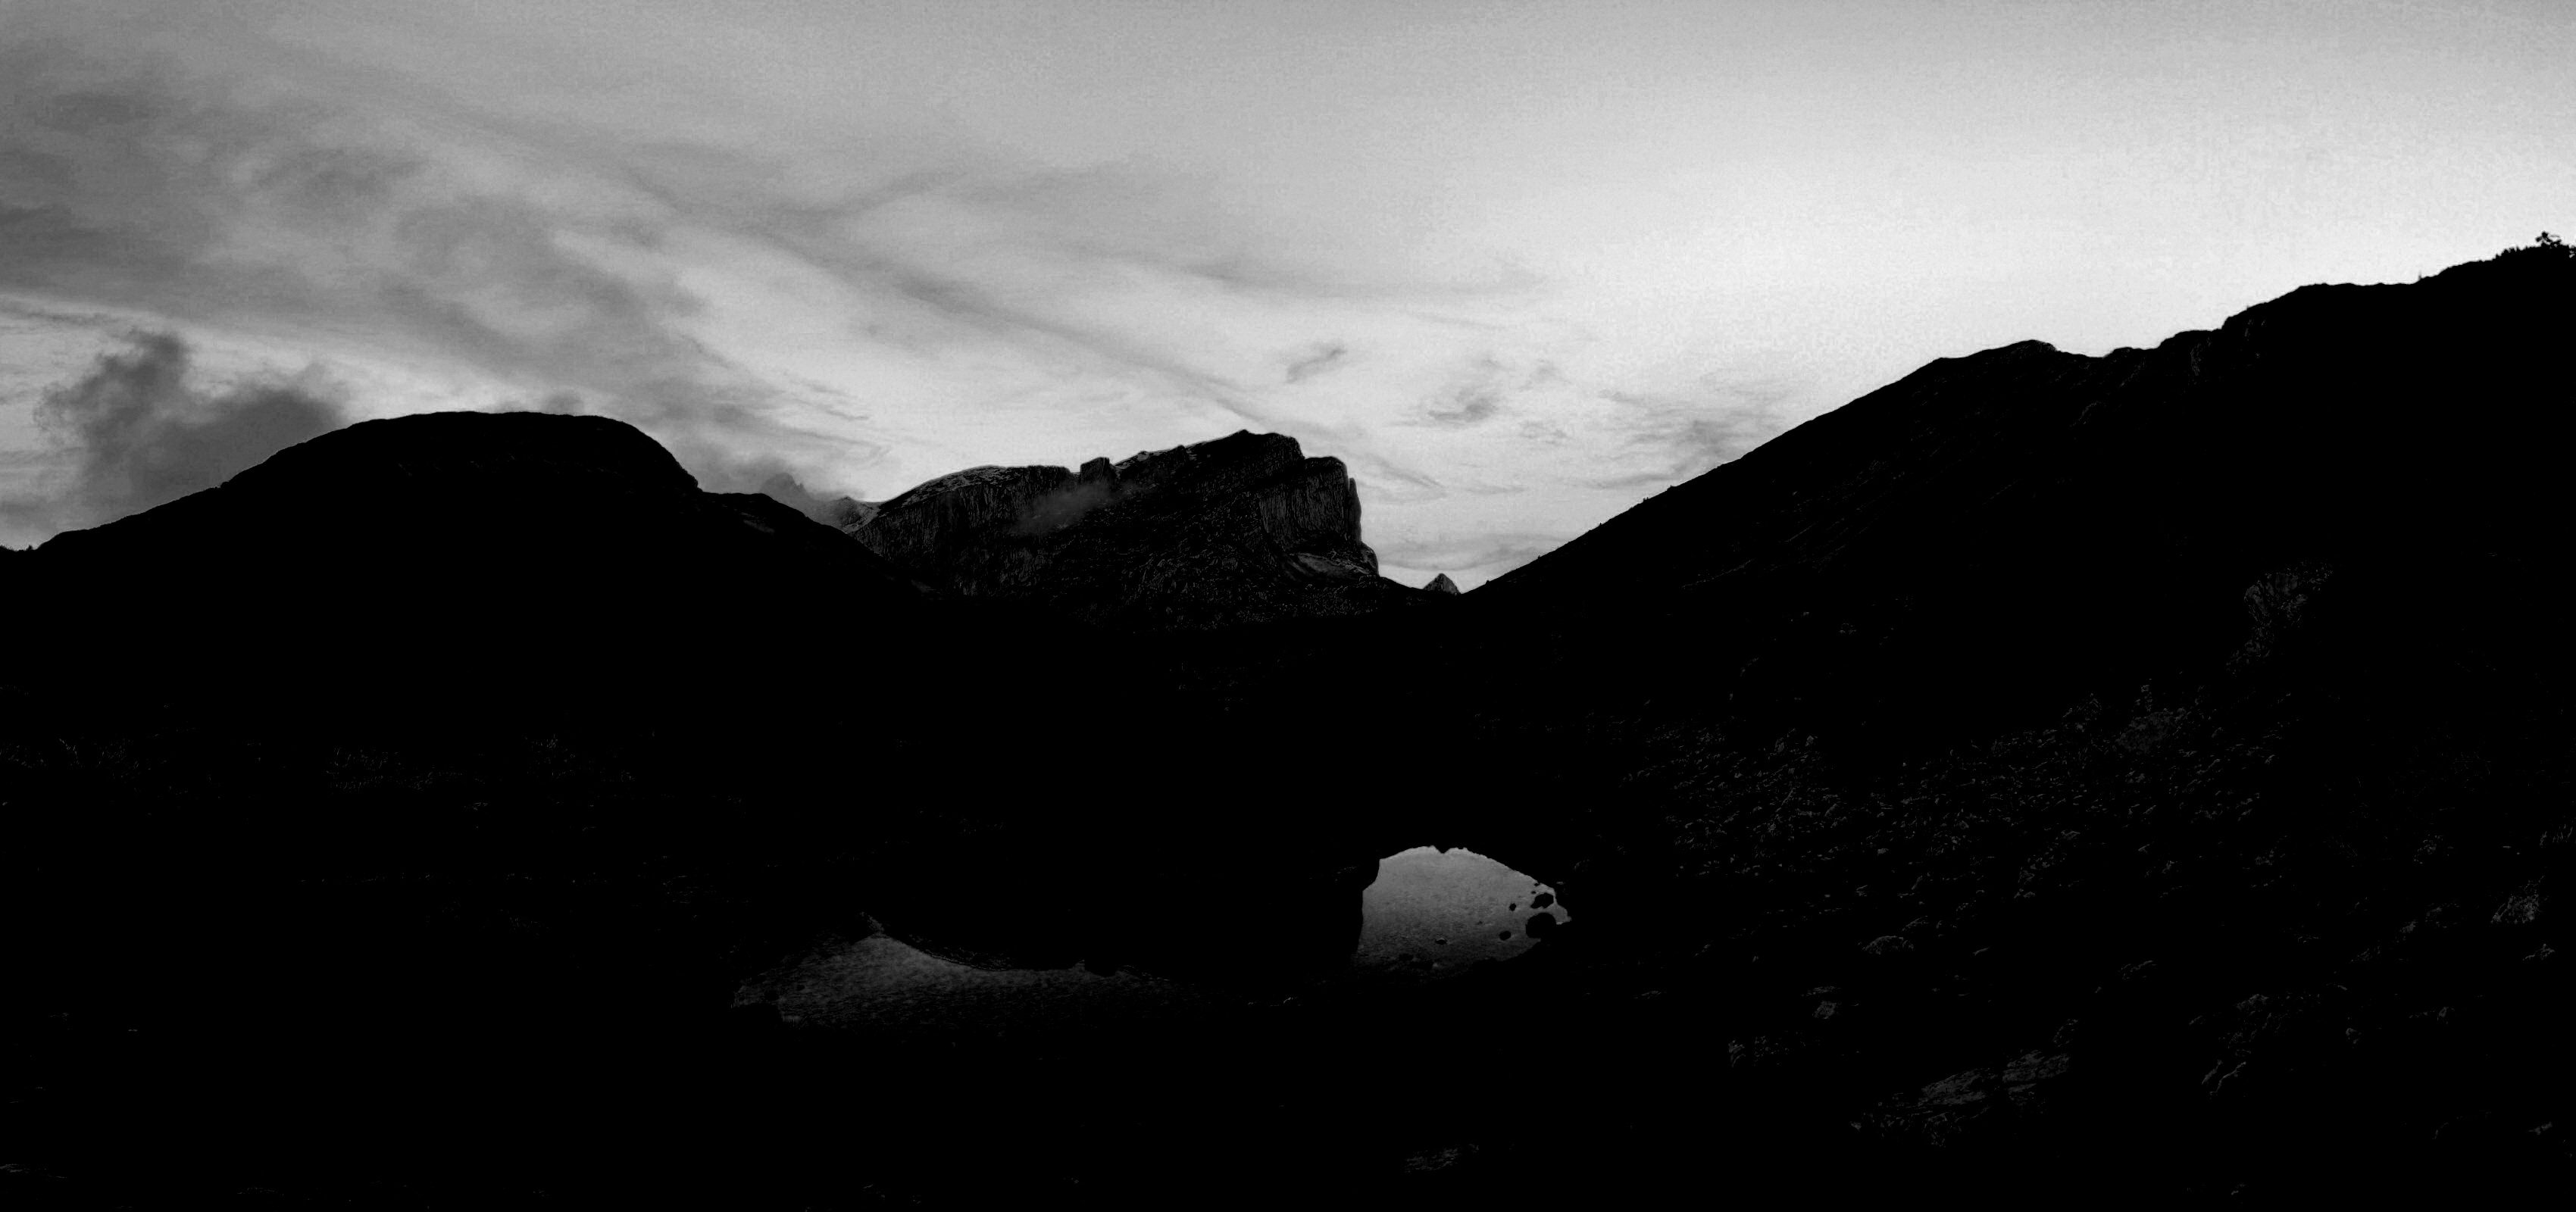
\includegraphics[width=\textwidth]{../Bilder/Sky_Blackening_FirstStep.jpg}
\subcaption{Kontrasttransformiertes Bild}
\label{simg:Trans}
\end{subfigure}
%
\begin{subfigure}[c]{0.9\textwidth}
% This file has been created by Matfig2PGF v0.3.9
\begin{pgfpicture}
  % Axes
  \begin{pgfscope}
    \definecolor{matfig2pgf_color}{rgb}{1,1,1}\pgfsetfillcolor{matfig2pgf_color}
    \pgfpathrectangle{\pgfpoint{2.07868cm}{0.242746cm}}{\pgfpoint{13.4881cm}{6.3955cm}}
    \pgfusepath{fill}
  \end{pgfscope}
  % Grid
  \begin{pgfscope}
    \pgfsetlinewidth{0.5pt}
    \pgfsetdash{{\pgflinewidth}{0.5mm}}{0pt}
    \foreach \x in {2.70334,5.01691,7.33048,9.64404,11.9576,14.2712}
    {
      \pgfpathmoveto{\pgfpoint{\x cm}{0.242746cm}}\pgfpathlineto{\pgfpoint{\x cm}{6.63824cm}}
    }
    \foreach \y in {0.242746,0.953357,1.66397,2.37458,3.08519,3.7958,4.50641,5.21702,5.92763,6.63824}
    {
      \pgfpathmoveto{\pgfpoint{2.07868cm}{\y cm}}\pgfpathlineto{\pgfpoint{15.5668cm}{\y cm}}
    }
    \pgfusepath{stroke}
  \end{pgfscope}
  % X tick marks
  \begin{pgfscope}
    \pgfsetlinewidth{0.5pt}
    \definecolor{matfig2pgf_linecolor}{rgb}{0.000,0.000,0.000}
    \pgfsetstrokecolor{matfig2pgf_linecolor}
    \foreach \x in {2.70334,5.01691,7.33048,9.64404,11.9576,14.2712}
    {
      \pgfpathmoveto{\pgfpoint{\x cm}{0.242746cm}}\pgfpathlineto{\pgfpoint{\x cm}{0.306701cm}}
    }
    \pgfusepath{stroke}
  \end{pgfscope}
  % Y tick marks
  \begin{pgfscope}
    \pgfsetlinewidth{0.5pt}
    \definecolor{matfig2pgf_linecolor}{rgb}{0.000,0.000,0.000}
    \pgfsetstrokecolor{matfig2pgf_linecolor}
    \foreach \y in {0.242746,0.953357,1.66397,2.37458,3.08519,3.7958,4.50641,5.21702,5.92763,6.63824}
    {
      \pgfpathmoveto{\pgfpoint{2.07868cm}{\y cm}}\pgfpathlineto{\pgfpoint{2.21356cm}{\y cm}}
    }
    \pgfusepath{stroke}
  \end{pgfscope}
  % Outer axes line
  \begin{pgfscope}
    \pgfsetlinewidth{0.5pt}
    \definecolor{matfig2pgf_linecolor}{rgb}{0.000,0.000,0.000}
    \pgfsetstrokecolor{matfig2pgf_linecolor}
    \pgfpathmoveto{\pgfpoint{2.078679cm}{0.242746cm}}\pgfpathlineto{\pgfpoint{15.566776cm}{0.242746cm}}
    \pgfusepath{stroke}
  \end{pgfscope}
  \begin{pgfscope}
    \pgfsetlinewidth{0.5pt}
    \definecolor{matfig2pgf_linecolor}{rgb}{0.000,0.000,0.000}
    \pgfsetstrokecolor{matfig2pgf_linecolor}
    \pgfpathmoveto{\pgfpoint{2.078679cm}{0.242746cm}}\pgfpathlineto{\pgfpoint{2.078679cm}{6.638244cm}}
    \pgfusepath{stroke}
  \end{pgfscope}
  % Tick labels
  \begin{pgfscope}
    \definecolor{matfig2pgf_fillcolor}{rgb}{0.000,0.000,0.000}
    \pgfsetfillcolor{matfig2pgf_fillcolor}
    \pgftext[x=2.70334cm,y=0.142746cm,top]{$-300$}
    \pgftext[x=5.01691cm,y=0.142746cm,top]{$-200$}
    \pgftext[x=7.33048cm,y=0.142746cm,top]{$-100$}
    \pgftext[x=9.64404cm,y=0.142746cm,top]{$0$}
    \pgftext[x=11.9576cm,y=0.142746cm,top]{$100$}
    \pgftext[x=14.2712cm,y=0.142746cm,top]{$200$}
  \end{pgfscope}
  % Line
  \makeatletter\ifpgf@draftmode\makeatother\else
  \begin{pgfscope}
    \pgfpathrectangle{\pgfpoint{2.07868cm}{0.242746cm}}{\pgfpoint{13.4881cm}{6.3955cm}}
    \pgfusepath{clip}
    % Draw line part (line itself)
    \begin{pgfscope}
      \pgfsetlinewidth{1.50pt}
      \definecolor{matfig2pgf_linecolor}{rgb}{1.000,0.000,0.000}
      \pgfsetstrokecolor{matfig2pgf_linecolor}
      \pgfsetdash{}{0pt}
      \pgfsetroundjoin
      \pgfplothandlerlineto
\pgfplotstreamstart
\foreach \x/\y in {2.102/0.243,5.642/0.250,5.896/0.271,6.035/0.307,6.151/0.371,6.266/0.471,6.359/0.607,6.382/0.665,6.405/0.686
,6.544/1.061,6.636/1.445,6.660/1.512,6.729/1.869,6.845/2.609,6.983/3.684,7.007/3.795,7.076/4.403,7.122/4.652,7.145/4.834
,7.169/4.899,7.192/5.118,7.215/5.195,7.261/5.463,7.284/5.537,7.330/5.859,7.354/5.887,7.377/6.032,7.423/6.209,7.446/6.268
,7.469/6.376,7.492/6.383,7.516/6.493,7.562/6.433,7.585/6.558,7.608/6.579,7.631/6.578,7.678/6.502,7.724/6.381,7.747/6.345
,7.770/6.234,7.793/6.006,7.816/5.935,7.839/5.698,7.863/5.589,7.909/5.184,7.955/4.826,7.978/4.810,8.001/4.456,8.025/4.451
,8.048/4.272,8.094/4.187,8.117/4.039,8.140/4.153,8.163/3.970,8.186/4.175,8.210/4.151,8.233/3.993,8.256/4.226,8.279/4.284
,8.302/4.154,8.325/4.486,8.348/4.320,8.372/4.481,8.418/4.257,8.441/4.290,8.464/3.928,8.487/3.845,8.510/3.434,8.557/3.065
,8.580/2.794,8.649/2.412,8.672/2.214,8.719/2.109,8.742/1.956,8.765/1.909,8.834/1.674,8.857/1.647,8.881/1.548,8.904/1.508
,8.927/1.486,8.950/1.404,8.973/1.382,8.996/1.319,9.019/1.285,9.066/1.279,9.112/1.180,9.135/1.214,9.158/1.150,9.181/1.133
,9.204/1.144,9.274/1.097,9.297/1.068,9.320/1.086,9.390/1.060,9.413/1.100,9.459/1.045,9.505/1.089,9.528/1.064,9.552/1.077
,9.575/1.052,9.598/1.062,9.621/1.041,9.644/1.039,9.667/1.765,9.690/0.983,9.760/0.952,9.783/0.927,9.829/0.941,9.875/0.866
,9.899/0.881,9.922/0.867,9.945/0.831,9.968/0.864,9.991/0.812,10.014/0.813,10.037/0.779,10.060/0.767,10.084/0.737,10.107/0.740
,10.153/0.696,10.176/0.714,10.199/0.683,10.222/0.677,10.246/0.648,10.269/0.655,10.292/0.625,10.315/0.613,10.361/0.571,10.454/0.506
,10.477/0.473,10.500/0.477,10.523/0.459,10.546/0.453,10.593/0.420,10.639/0.420,10.662/0.392,10.685/0.395,10.708/0.373,10.755/0.374
,10.801/0.349,10.870/0.329,10.893/0.331,10.917/0.322,11.125/0.308,11.148/0.315,11.194/0.302,11.264/0.305,11.287/0.301,11.310/0.325
,11.333/0.328,11.356/0.362,11.402/0.374,11.472/0.482,11.495/0.536,11.518/0.525,11.541/0.600,11.564/0.566,11.587/0.508,11.611/0.535
,11.634/0.514,11.657/0.463,11.703/0.478,11.749/0.535,11.773/0.576,11.796/0.584,11.865/0.684,11.911/0.708,11.934/0.758,11.958/0.779
,11.981/0.773,12.004/0.865,12.027/0.701,12.050/0.684,12.073/0.751,12.096/0.782,12.120/0.738,12.143/0.895,12.166/0.911,12.189/0.883
,12.235/0.873,12.258/0.812,12.282/0.866,12.305/0.887,12.351/0.810,12.374/0.891,12.397/0.795,12.420/0.860,12.490/0.832,12.513/0.875
,12.559/1.007,12.582/1.028,12.605/1.106,12.629/1.153,12.652/1.119,12.675/1.217,12.698/1.205,12.721/1.155,12.744/1.248,12.767/1.212
,12.837/1.487,12.860/1.605,12.883/1.609,12.906/1.693,12.929/1.625,12.952/1.681,12.976/1.705,12.999/1.754,13.022/1.751,13.045/1.690
,13.068/1.711,13.091/1.791,13.114/1.805,13.138/2.025,13.161/1.770,13.184/1.911,13.207/1.683,13.230/1.876,13.253/1.780,13.276/1.766
,13.299/1.887,13.323/1.838,13.346/1.977,13.392/1.966,13.415/2.106,13.438/2.393,13.461/2.402,13.485/2.481,13.508/2.730,13.531/2.786
,13.554/2.926,13.577/2.806,13.600/3.251,13.623/2.874,13.647/3.239,13.670/2.800,13.693/3.282,13.716/2.707,13.739/2.923,13.762/2.715
,13.808/2.516,13.832/2.784,13.855/2.541,13.878/2.984,13.901/2.679,13.947/3.115,13.970/2.916,13.994/2.817,14.017/2.592,14.040/2.940
,14.086/2.439,14.109/2.639,14.132/2.620,14.179/2.961,14.202/2.702,14.225/3.079,14.248/2.874,14.271/2.826,14.294/2.968,14.317/2.582
,14.341/2.731,14.364/2.672,14.387/2.534,14.410/2.813,14.433/2.468,14.456/2.776,14.479/2.610,14.503/2.711,14.526/2.565,14.549/2.815
,14.572/2.758,14.595/2.637,14.618/2.684,14.641/2.398,14.664/2.441,14.688/2.154,14.711/2.379,14.734/2.201,14.757/2.165,14.780/2.181
,14.803/2.420,14.826/2.360,14.850/2.717,14.873/2.886,14.896/3.291,14.919/3.010,14.942/3.228,14.965/3.019,14.988/2.482,15.012/2.593
,15.035/2.231,15.081/2.024,15.104/1.607,15.127/1.621,15.150/0.989,15.173/0.882,15.197/0.609,15.220/0.524,15.243/0.358,15.289/0.271
,15.335/0.250,15.590/0.243}
{
\pgfplotstreampoint{\pgfpoint{\x cm}{\y cm}}
}
\pgfplotstreamend
      \pgfusepath{stroke}
    \end{pgfscope}
  \end{pgfscope}
  \fi
  \makeatletter\ifpgf@draftmode\makeatother\pgftext[x=7.99492cm,y=3.44049cm]{\Huge{DRAFT}}\fi
\end{pgfpicture}

\subcaption{Kontrasttransformiertes Histogramm}
\label{simg:Hist}
\end{subfigure}
\caption[Kontrasttransformation für sky blackening]{Kontrasttransformation einer Landschaftsaufnahme. (a) zeigt das Originalbild, (b) das transformierte Bild und (c) das Histogramm des Transformationsbildes. Das Bild stammt von \url{https://commons.wikimedia.org/w/index.php?curid=1262156} (fotografiert und hochgeladen von Karsten Dörre)}\label{img:sky_Trans}
\end{figure} 
Damit die standardisierten Bildverarbeitungsalgorithmen auf dieses Histogramm angewendet werden können, müssen die Werte noch in einen 8-Bit Grauwertbereich transformiert werden. Hierfür kann entweder das Autoscaling"=Verfahren angewendet werden, oder die Histogrammwerte links und rechts der unteren und oberen Grauwertgrenze abgeschnitten werden. 

In diesem Fall wurde das Histogramm auf einen bestimmten Bereich zugeschnitten. Grauwerte, die sich außerhalb der Bereiche befanden wurden auf den am nächsten liegenden Grenzwert transformiert. Somit wird beinahe der komplette Vordergrund im so entstandenen Bild schwarz, während der Himmelsbereich in helleren Grauwertstufen dargestellt wird (siehe \autoref{simg:Trans}). Anschließend folgt die Segmentation des Himmels.

\begin{figure}[h!]
\centering
\resizebox{0.9\textwidth}{6cm}{% This file has been created by Matfig2PGF v0.3.9
\begin{pgfpicture}
  % Axes
  \begin{pgfscope}
    \definecolor{matfig2pgf_color}{rgb}{1,1,1}\pgfsetfillcolor{matfig2pgf_color}
    \pgfpathrectangle{\pgfpoint{1.69226cm}{1.27196cm}}{\pgfpoint{13.9591cm}{6.17227cm}}
    \pgfusepath{fill}
  \end{pgfscope}
  % Grid
  \begin{pgfscope}
    \pgfsetlinewidth{0.5pt}
    \pgfsetdash{{\pgflinewidth}{0.5mm}}{0pt}
    \foreach \x in {1.72365,4.46086,7.19808,9.93529,12.6725,15.4097}
    {
      \pgfpathmoveto{\pgfpoint{\x cm}{1.27196cm}}\pgfpathlineto{\pgfpoint{\x cm}{7.44423cm}}
    }
    \foreach \y in {1.2905,2.06385,2.8372,3.61055,4.3839,5.15725,5.9306,6.70395}
    {
      \pgfpathmoveto{\pgfpoint{1.69226cm}{\y cm}}\pgfpathlineto{\pgfpoint{15.6514cm}{\y cm}}
    }
    \pgfusepath{stroke}
  \end{pgfscope}
  % X tick marks
  \begin{pgfscope}
    \pgfsetlinewidth{0.5pt}
    \definecolor{matfig2pgf_linecolor}{rgb}{0.000,0.000,0.000}
    \pgfsetstrokecolor{matfig2pgf_linecolor}
    \foreach \x in {1.72365,4.46086,7.19808,9.93529,12.6725,15.4097}
    {
      \pgfpathmoveto{\pgfpoint{\x cm}{1.27196cm}}\pgfpathlineto{\pgfpoint{\x cm}{1.33368cm}}
    }
    \pgfusepath{stroke}
  \end{pgfscope}
  % Y tick marks
  \begin{pgfscope}
    \pgfsetlinewidth{0.5pt}
    \definecolor{matfig2pgf_linecolor}{rgb}{0.000,0.000,0.000}
    \pgfsetstrokecolor{matfig2pgf_linecolor}
    \foreach \y in {1.2905,2.06385,2.8372,3.61055,4.3839,5.15725,5.9306,6.70395}
    {
      \pgfpathmoveto{\pgfpoint{1.69226cm}{\y cm}}\pgfpathlineto{\pgfpoint{1.83185cm}{\y cm}}
    }
    \pgfusepath{stroke}
  \end{pgfscope}
  % Outer axes line
  \begin{pgfscope}
    \pgfsetlinewidth{0.5pt}
    \definecolor{matfig2pgf_linecolor}{rgb}{0.000,0.000,0.000}
    \pgfsetstrokecolor{matfig2pgf_linecolor}
    \pgfpathmoveto{\pgfpoint{1.692258cm}{1.271959cm}}\pgfpathlineto{\pgfpoint{15.651389cm}{1.271959cm}}
    \pgfusepath{stroke}
  \end{pgfscope}
  \begin{pgfscope}
    \pgfsetlinewidth{0.5pt}
    \definecolor{matfig2pgf_linecolor}{rgb}{0.000,0.000,0.000}
    \pgfsetstrokecolor{matfig2pgf_linecolor}
    \pgfpathmoveto{\pgfpoint{1.692258cm}{1.271959cm}}\pgfpathlineto{\pgfpoint{1.692258cm}{7.444226cm}}
    \pgfusepath{stroke}
  \end{pgfscope}
  % Tick labels
  \begin{pgfscope}
    \definecolor{matfig2pgf_fillcolor}{rgb}{0.000,0.000,0.000}
    \pgfsetfillcolor{matfig2pgf_fillcolor}
    \pgftext[x=1.72365cm,y=1.17196cm,top]{$0$}
    \pgftext[x=4.46086cm,y=1.17196cm,top]{$50$}
    \pgftext[x=7.19808cm,y=1.17196cm,top]{$100$}
    \pgftext[x=9.93529cm,y=1.17196cm,top]{$150$}
    \pgftext[x=12.6725cm,y=1.17196cm,top]{$200$}
    \pgftext[x=15.4097cm,y=1.17196cm,top]{$250$}
  \end{pgfscope}
  % Line
  \makeatletter\ifpgf@draftmode\makeatother\else
  \begin{pgfscope}
    \pgfpathrectangle{\pgfpoint{1.69226cm}{1.27196cm}}{\pgfpoint{13.9591cm}{6.17227cm}}
    \pgfusepath{clip}
    % Draw line part (line itself)
    \begin{pgfscope}
      \pgfsetlinewidth{1.50pt}
      \definecolor{matfig2pgf_linecolor}{rgb}{1.000,0.000,0.000}
      \pgfsetstrokecolor{matfig2pgf_linecolor}
      \pgfsetdash{}{0pt}
      \pgfsetroundjoin
      \pgfplothandlerlineto
\pgfplotstreamstart
\foreach \x/\y in {1.724/15.567,1.778/2.096,1.943/2.063,1.997/2.036,2.107/2.051,2.216/1.968,2.271/1.985,2.326/1.970,2.381/1.931
,2.435/1.966,2.490/1.910,2.545/1.911,2.600/1.874,2.654/1.861,2.709/1.829,2.764/1.832,2.873/1.784,2.928/1.804,2.983/1.770
,3.038/1.763,3.092/1.731,3.147/1.739,3.202/1.706,3.256/1.694,3.311/1.665,3.585/1.577,3.640/1.541,3.694/1.546,3.749/1.525
,3.804/1.520,3.913/1.483,4.023/1.483,4.078/1.453,4.132/1.457,4.187/1.433,4.297/1.433,4.406/1.406,4.570/1.385,4.625/1.387
,4.680/1.377,4.954/1.366,5.173/1.362,5.227/1.369,5.337/1.354,5.501/1.358,5.556/1.354,5.610/1.379,5.665/1.383,5.720/1.420
,5.829/1.434,5.884/1.482,5.994/1.551,6.048/1.610,6.103/1.598,6.158/1.679,6.213/1.643,6.267/1.580,6.322/1.609,6.377/1.585
,6.432/1.530,6.541/1.547,6.596/1.569,6.705/1.653,6.760/1.662,6.924/1.771,6.979/1.777,7.034/1.797,7.089/1.851,7.143/1.874
,7.198/1.868,7.253/1.968,7.308/1.789,7.362/1.771,7.417/1.844,7.472/1.877,7.527/1.829,7.581/2.000,7.636/2.018,7.691/1.987
,7.746/1.988,7.800/1.976,7.855/1.910,7.910/1.969,7.964/1.991,8.074/1.908,8.129/1.996,8.183/1.892,8.238/1.962,8.402/1.932
,8.457/1.979,8.512/2.063,8.567/2.123,8.621/2.145,8.676/2.230,8.731/2.281,8.786/2.244,8.840/2.350,8.895/2.338,8.950/2.284
,9.005/2.385,9.059/2.345,9.114/2.423,9.224/2.645,9.278/2.773,9.333/2.777,9.388/2.869,9.443/2.795,9.497/2.856,9.552/2.882
,9.607/2.936,9.662/2.931,9.716/2.866,9.771/2.889,9.826/2.975,9.881/2.991,9.935/3.230,9.990/2.953,10.045/3.106,10.100/2.858
,10.154/3.068,10.209/2.963,10.264/2.949,10.319/3.080,10.373/3.027,10.428/3.178,10.537/3.166,10.592/3.318,10.647/3.630,10.702/3.640
,10.756/3.726,10.811/3.997,10.866/4.059,10.921/4.210,10.975/4.080,11.030/4.564,11.085/4.154,11.140/4.551,11.194/4.074,11.249/4.598
,11.304/3.973,11.359/4.207,11.413/3.981,11.468/3.850,11.523/3.764,11.578/4.056,11.632/3.792,11.687/4.274,11.742/3.942,11.797/4.131
,11.851/4.417,11.906/4.200,11.961/4.092,12.016/3.847,12.070/4.226,12.180/3.681,12.235/3.898,12.289/3.877,12.344/4.095,12.399/4.248
,12.454/3.967,12.508/4.378,12.563/4.154,12.618/4.102,12.673/4.256,12.727/3.837,12.782/3.999,12.837/3.934,12.891/3.784,12.946/4.087
,13.001/3.712,13.056/4.047,13.110/3.867,13.165/3.977,13.220/3.818,13.275/4.090,13.329/4.028,13.384/3.896,13.439/3.947,13.494/3.636
,13.548/3.683,13.603/3.370,13.658/3.616,13.713/3.422,13.767/3.382,13.822/3.400,13.877/3.659,13.932/3.595,13.986/3.983,14.041/4.167
,14.096/4.608,14.151/4.302,14.205/4.539,14.260/4.312,14.315/3.728,14.370/3.848,14.424/3.454,14.534/3.229,14.589/2.775,14.643/2.790
,14.698/2.102,14.753/1.986,14.808/1.689,14.862/1.597,14.917/1.416,15.027/1.321,15.136/1.298,15.683/1.291}
{
\pgfplotstreampoint{\pgfpoint{\x cm}{\y cm}}
}
\pgfplotstreamend
      \pgfusepath{stroke}
    \end{pgfscope}
  \end{pgfscope}
  \fi
  \makeatletter\ifpgf@draftmode\makeatother\pgftext[x=7.99492cm,y=3.89171cm]{\Huge{DRAFT}}\fi
\end{pgfpicture}
}
%\subfigure[Winkeldiagramm]{\resizebox{0.49\textwidth}{!}{\input{./Bilder/LF_Simple_Angle.pgf}}}
\caption[Histogrammtransformation]{Das Histogramm nach der Transformation auf den 8"=Bit Grauwertbereich. Alle Pixel, deren Werte vorher kleiner als $0$, sind nun genau auf der Nullachse. Daher verlässt das Histogramm an dieser Stelle den Wertebereich.}\label{img:Hist_cut}
%\vspace{-0.3 cm} % Abstand Bild -- Bildbeschriftung
\end{figure} 
%Verweis auf nachfolgendes Bild mit allen 4 Transformationsstufen
\subsubsection{Segmentation des Himmels}
Für die Segmentierung der Himmelsregion wird eine binäre Maske berechnet. Diese sorgt dafür, dass der Himmel komplett geschwärzt wird, während die restlichen Bereiche ihre alten Grauwerte beibehalten. Die Binärschwelle der Maske wird dabei automatisiert und angepasst an jedes einzelne Bild bestimmt. Das wohl bekannteste Verfahren zur Berechnung des Schwellwerts ist die sogenannte Otsu Methode \cite{otsu1975threshold}, die im folgenden kurz beschrieben werden soll.

Anschließend wird ein Schwellwert in das Histogramm gelegt, wodurch das Histogramm in zwei Klassen unterteilt wird. Für jede der beiden Klassen wird anschließend die gesamte Wahrscheinlichkeit, dass ein Pixel in dieser Klasse auftritt, und deren mittlerer Grauwert berechnet.
\begin{equation}
P_0(t)=\sum_{i=0}^{t}p_i\text{ und }P_1(t)=\sum_{i=t+1}^{255}p_i=1-P_0(t)
\end{equation}
\begin{equation}
\overline{g}_0=\frac{1}{P_0(t)}\sum_{i=0}^{t}p_i*i
\end{equation}
\begin{equation}
\overline{g}_1=\frac{1}{P_1(t)}\sum_{i=t+1}^{255}p_i*i
\end{equation}
Dabei ist $t$ der aktuelle Schwellwert, $P_0$ und $P_1$ sind die aufaddierten Häufigkeiten der beiden Klassen und $p(i)$ ist die Häufigkeit eines einzelnen Grauwerts. Das Ziel der Otsu Methode ist nun herauszufinden, bei welchem Schwellwert $t$ die Varianz innerhalb der Klassen minimal ist.
\begin{equation}
\sigma_i^2(t)=P_0(t)\sigma_0^2(t) + P_1\sigma_1^2(t)
\end{equation}
Bei $\sigma_0$ und $\sigma_1$ handelt es sich um die Varianzen innerhalb der beiden Klassen. 
\begin{equation}
\sigma_0^2=\frac{1}{P_0}\sum_{i=0}^t(i-\overline{g}_0)^2*p_i
\end{equation}
\begin{equation}
\sigma_1^2=\frac{1}{P_1}\sum_{i=t+1}^{255}(i-\overline{g}_1)^2*p_i
\end{equation}
Otsu hat jedoch gezeigt, dass die Stelle, an der die Varianz innerhalb der Klassen minimal ist, gleichzeitig auch die Stelle ist, an der die Varianz zwischen den beiden Klassen maximal ist. Da die Varianz zwischen den Klassen deutlich einfacher zu berechnen ist und auch programmatisch leichter umgesetzt werden kann, wird für die Otsu Methode meistens nur noch diese berechnet und nach dem maximalen Wert gesucht.
\begin{align}
\sigma_z^2(t)&=P_0(\overline{g}_0-\overline{g}_{ges})+P_1(\overline{g}_1-\overline{g}_{ges})\nonumber\\
&=P_0P_1(\overline{g}_0-\overline{g}_1)^2
\label{eqn:Var_zw_Otsu}
\end{align}
Aufgrund seiner Einfachheit und den sehr guten Ergebnissen, wird die Otsu Methode sehr oft für automatisierte Schwellwertdetektion eingesetzt. Der Nachteil besteht jedoch darin, dass sie nur bei bimodalen Grauwertverteilungen angewendet werden kann. Sollten jedoch nur sehr kleine Bereiche des Bildes dem Himmel oder dem Boden angehören, wird die vorherige Verteilung der Grauwerte annähernd unimodal. Daher wurde anstatt der Otsu Methode die sogenannte valley emphasis Methode angewendet. Hierbei sind alle Rechenschritte bis zu \autoref{eqn:Var_zw_Otsu} gleich. Bei der Berechnung der maximalen Varianz zwischen den Klassen wird jedoch noch eine Gewichtung $W$ hinzugefügt \cite{ng2006automatic}.
\begin{equation}
W=(1-p_t)
\end{equation}
Diese Gewichtung ist antiproportional zum Häufigkeitswert der aktuellen Schwelle. Dadurch werden die Ergebnisse für Schwellwerte in globalen Minima des Histogramms deutlich verbessert, während alle anderen Werte verschlechtert werden.
\begin{equation}
\sigma_z^2=W*P_0P_1(\overline{g}_0-\overline{g}_1)^2
\end{equation}
Wie zuvor wird nun nach dem Schwellwert gesucht, bei dem die gewichtete Varianz zwischen den Klassen maximal wird. Dieser wird anschließend zur Berechnung der Bildmaske verwendet. Dieses Verfahren kann jedoch nur bei Tagesaufnahmen. Bei Nachtaufnahmen ist das Verfahren nicht nötig, da hier der Himmel bereits schwarz erscheint. Sollten zudem Bilder in Gebäuden oder anderen Gegenden, wo kein Himmel zu sehen ist, aufgenommen werden, kann es ebenso nicht angewendet werden, da ansonsten Bildinformationen unnötig verloren gehen. 
%Bild mit verschiedenen Schritten zum sky blackening einfügen
\begin{figure}[h!]
\centering
\begin{subfigure}[c]{0.49\textwidth}
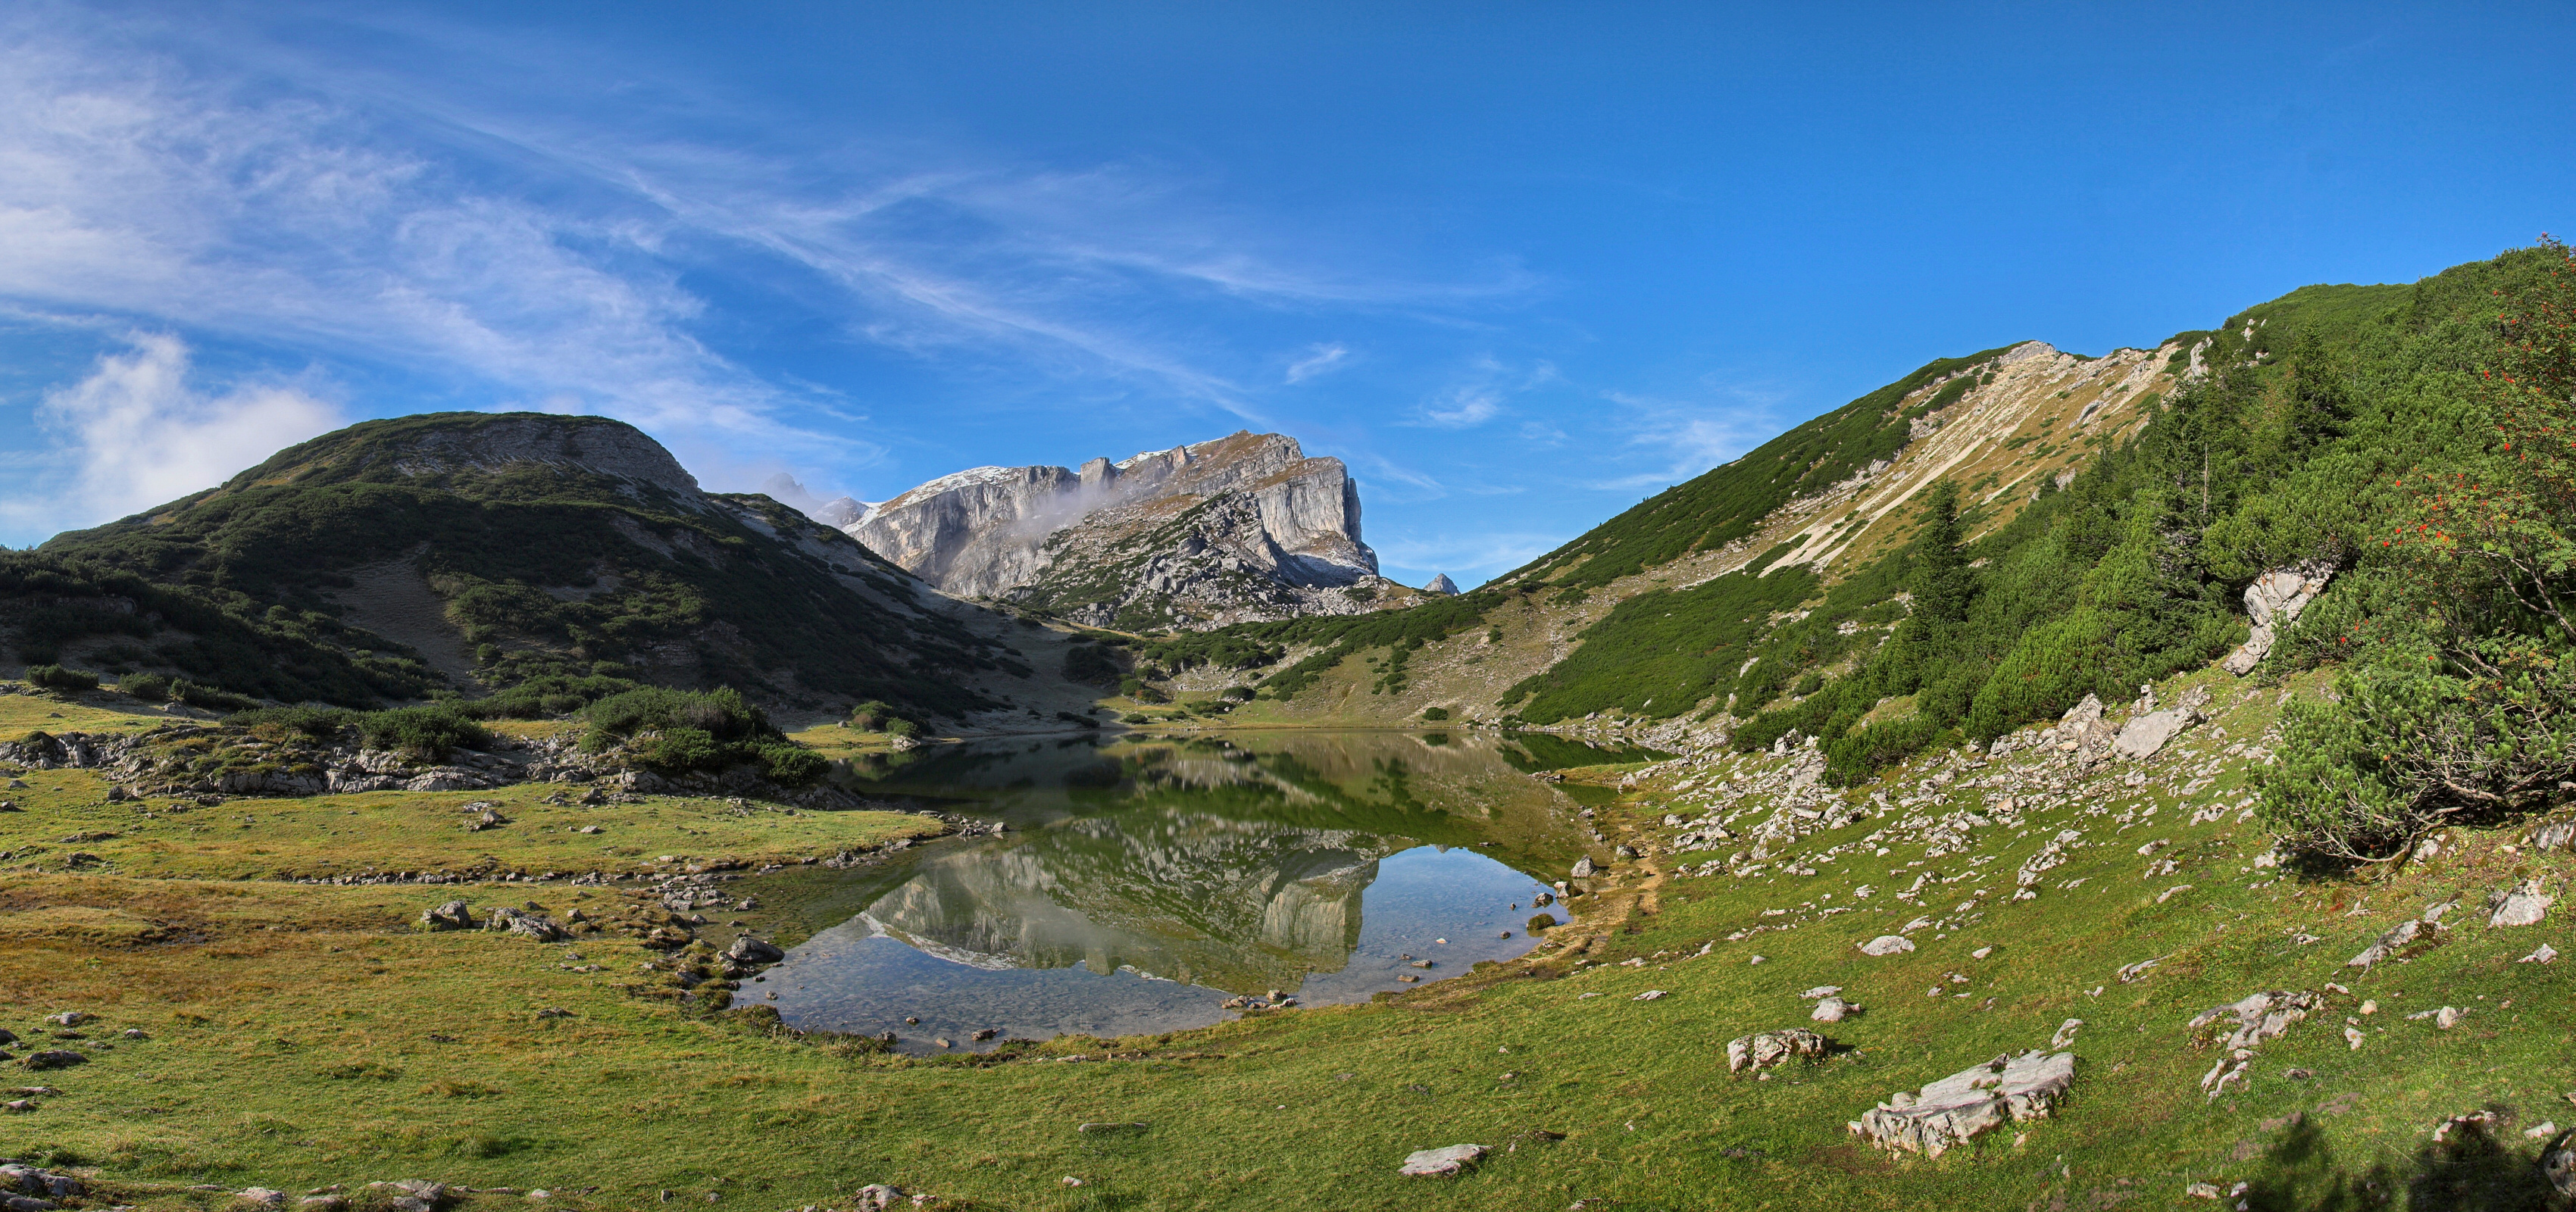
\includegraphics[width=\textwidth]{../Bilder/Zireiner_See_Rofanspitze_2006_10.jpg}
\subcaption{Originalbild}
\label{simg:Alle_Orig}
\end{subfigure}
%
\begin{subfigure}[c]{0.49\textwidth}
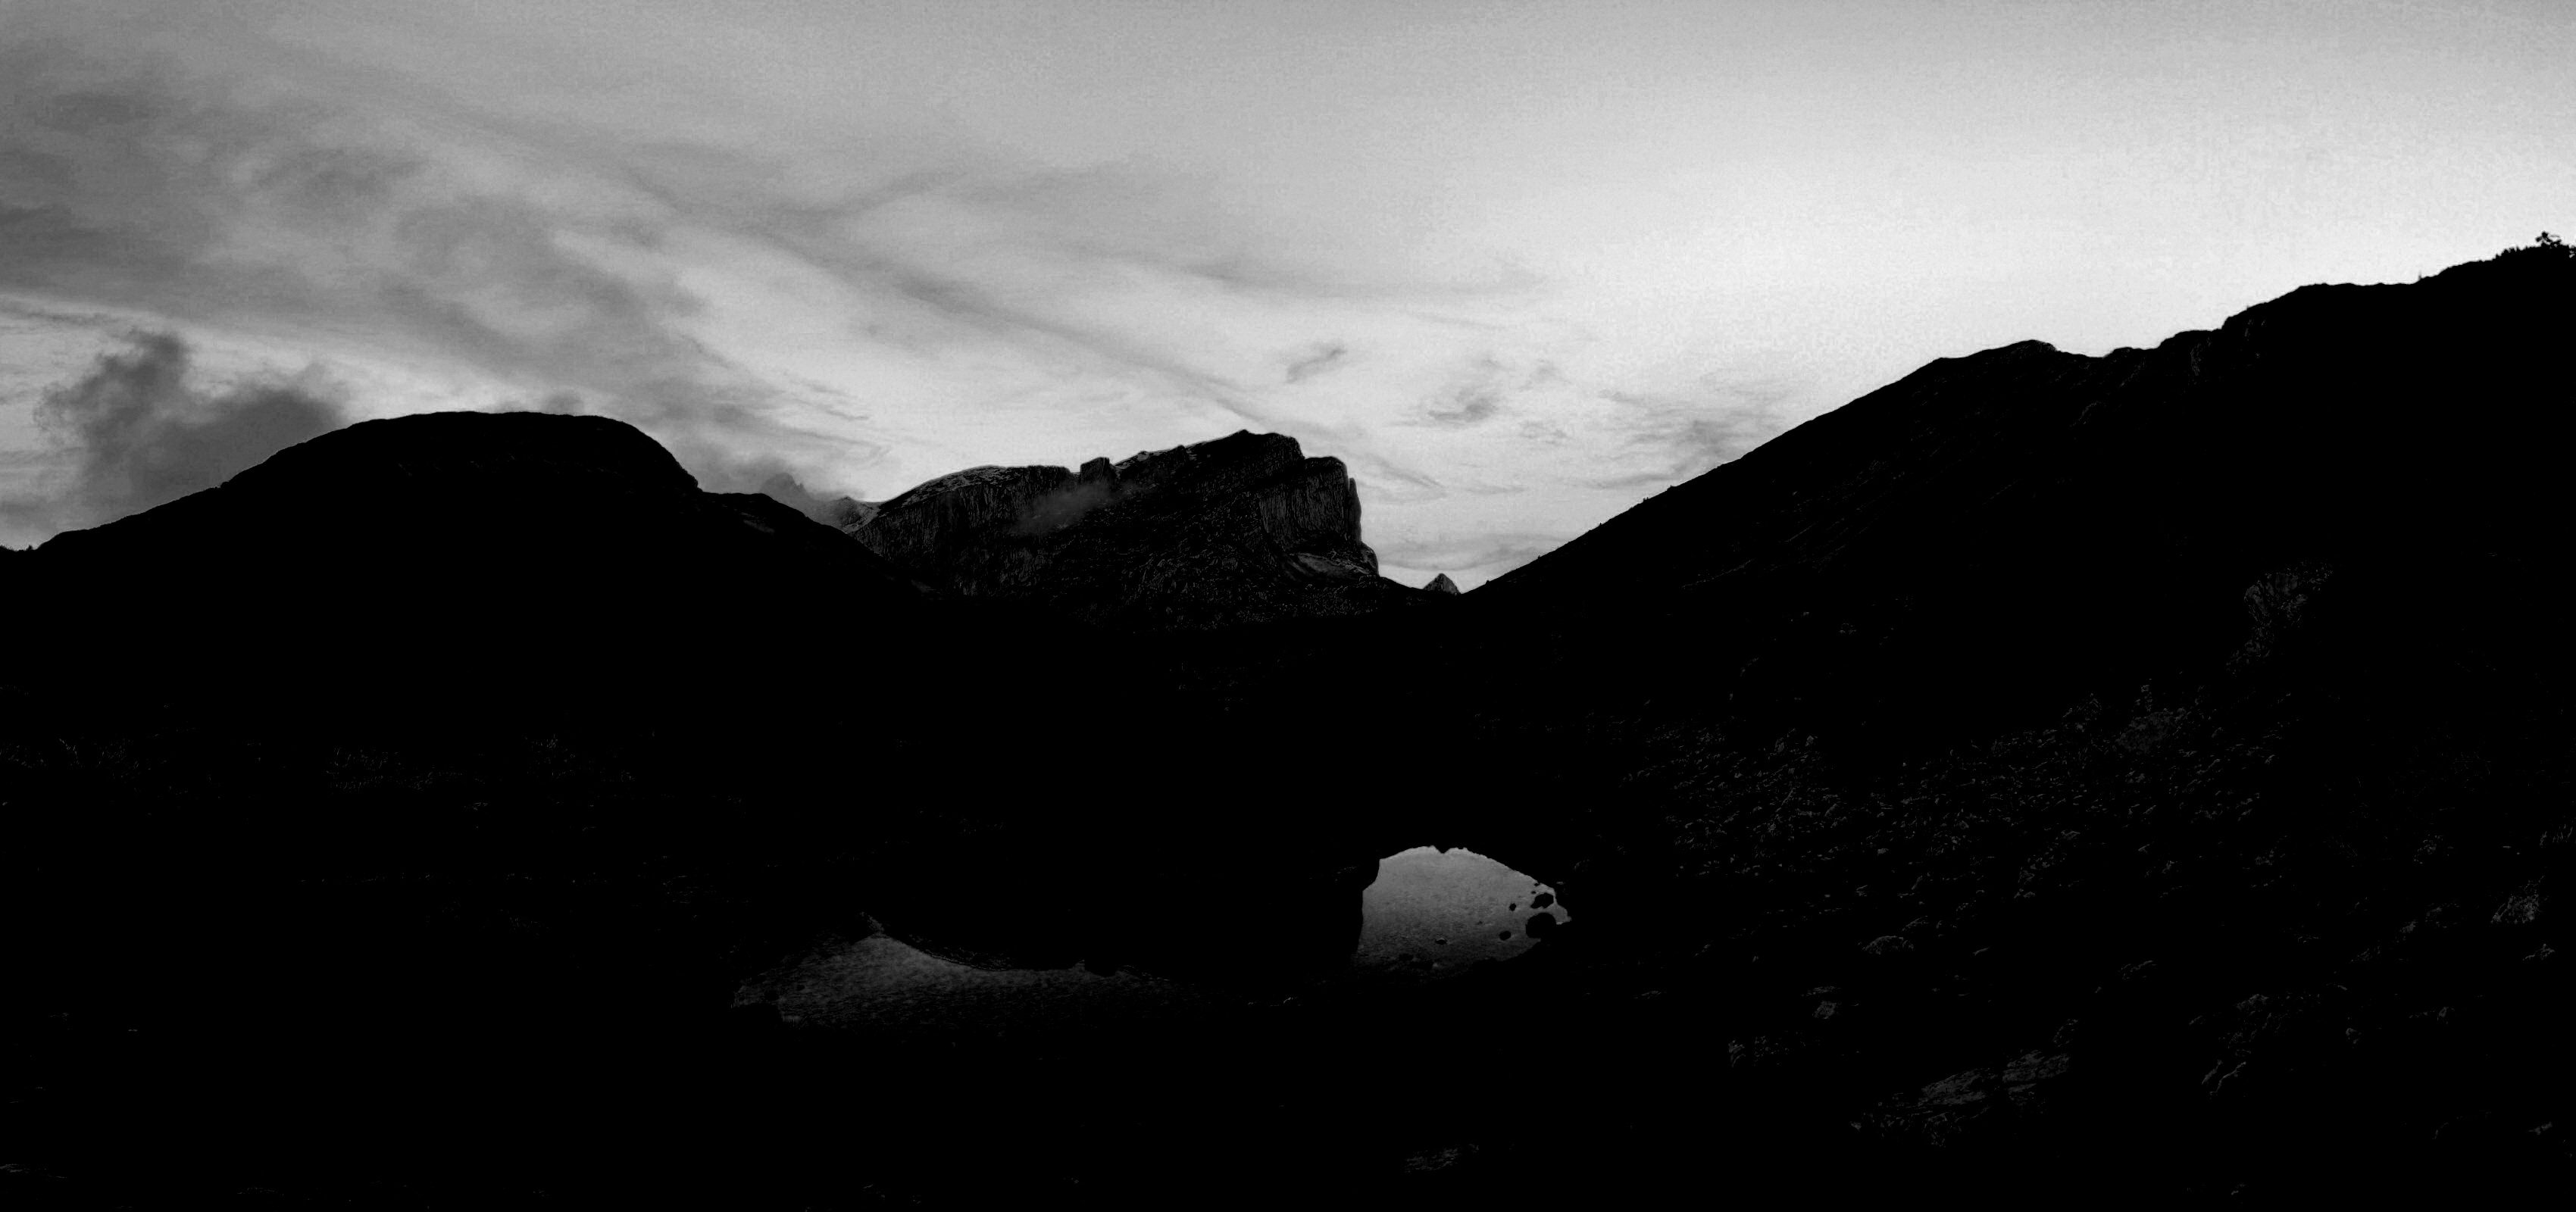
\includegraphics[width=\textwidth]{../Bilder/Sky_Blackening_FirstStep.jpg}
\subcaption{Kontrasttransformiertes Bild}
\label{simg:Alle_Trans}
\end{subfigure}
%
\begin{subfigure}[c]{0.49\textwidth}
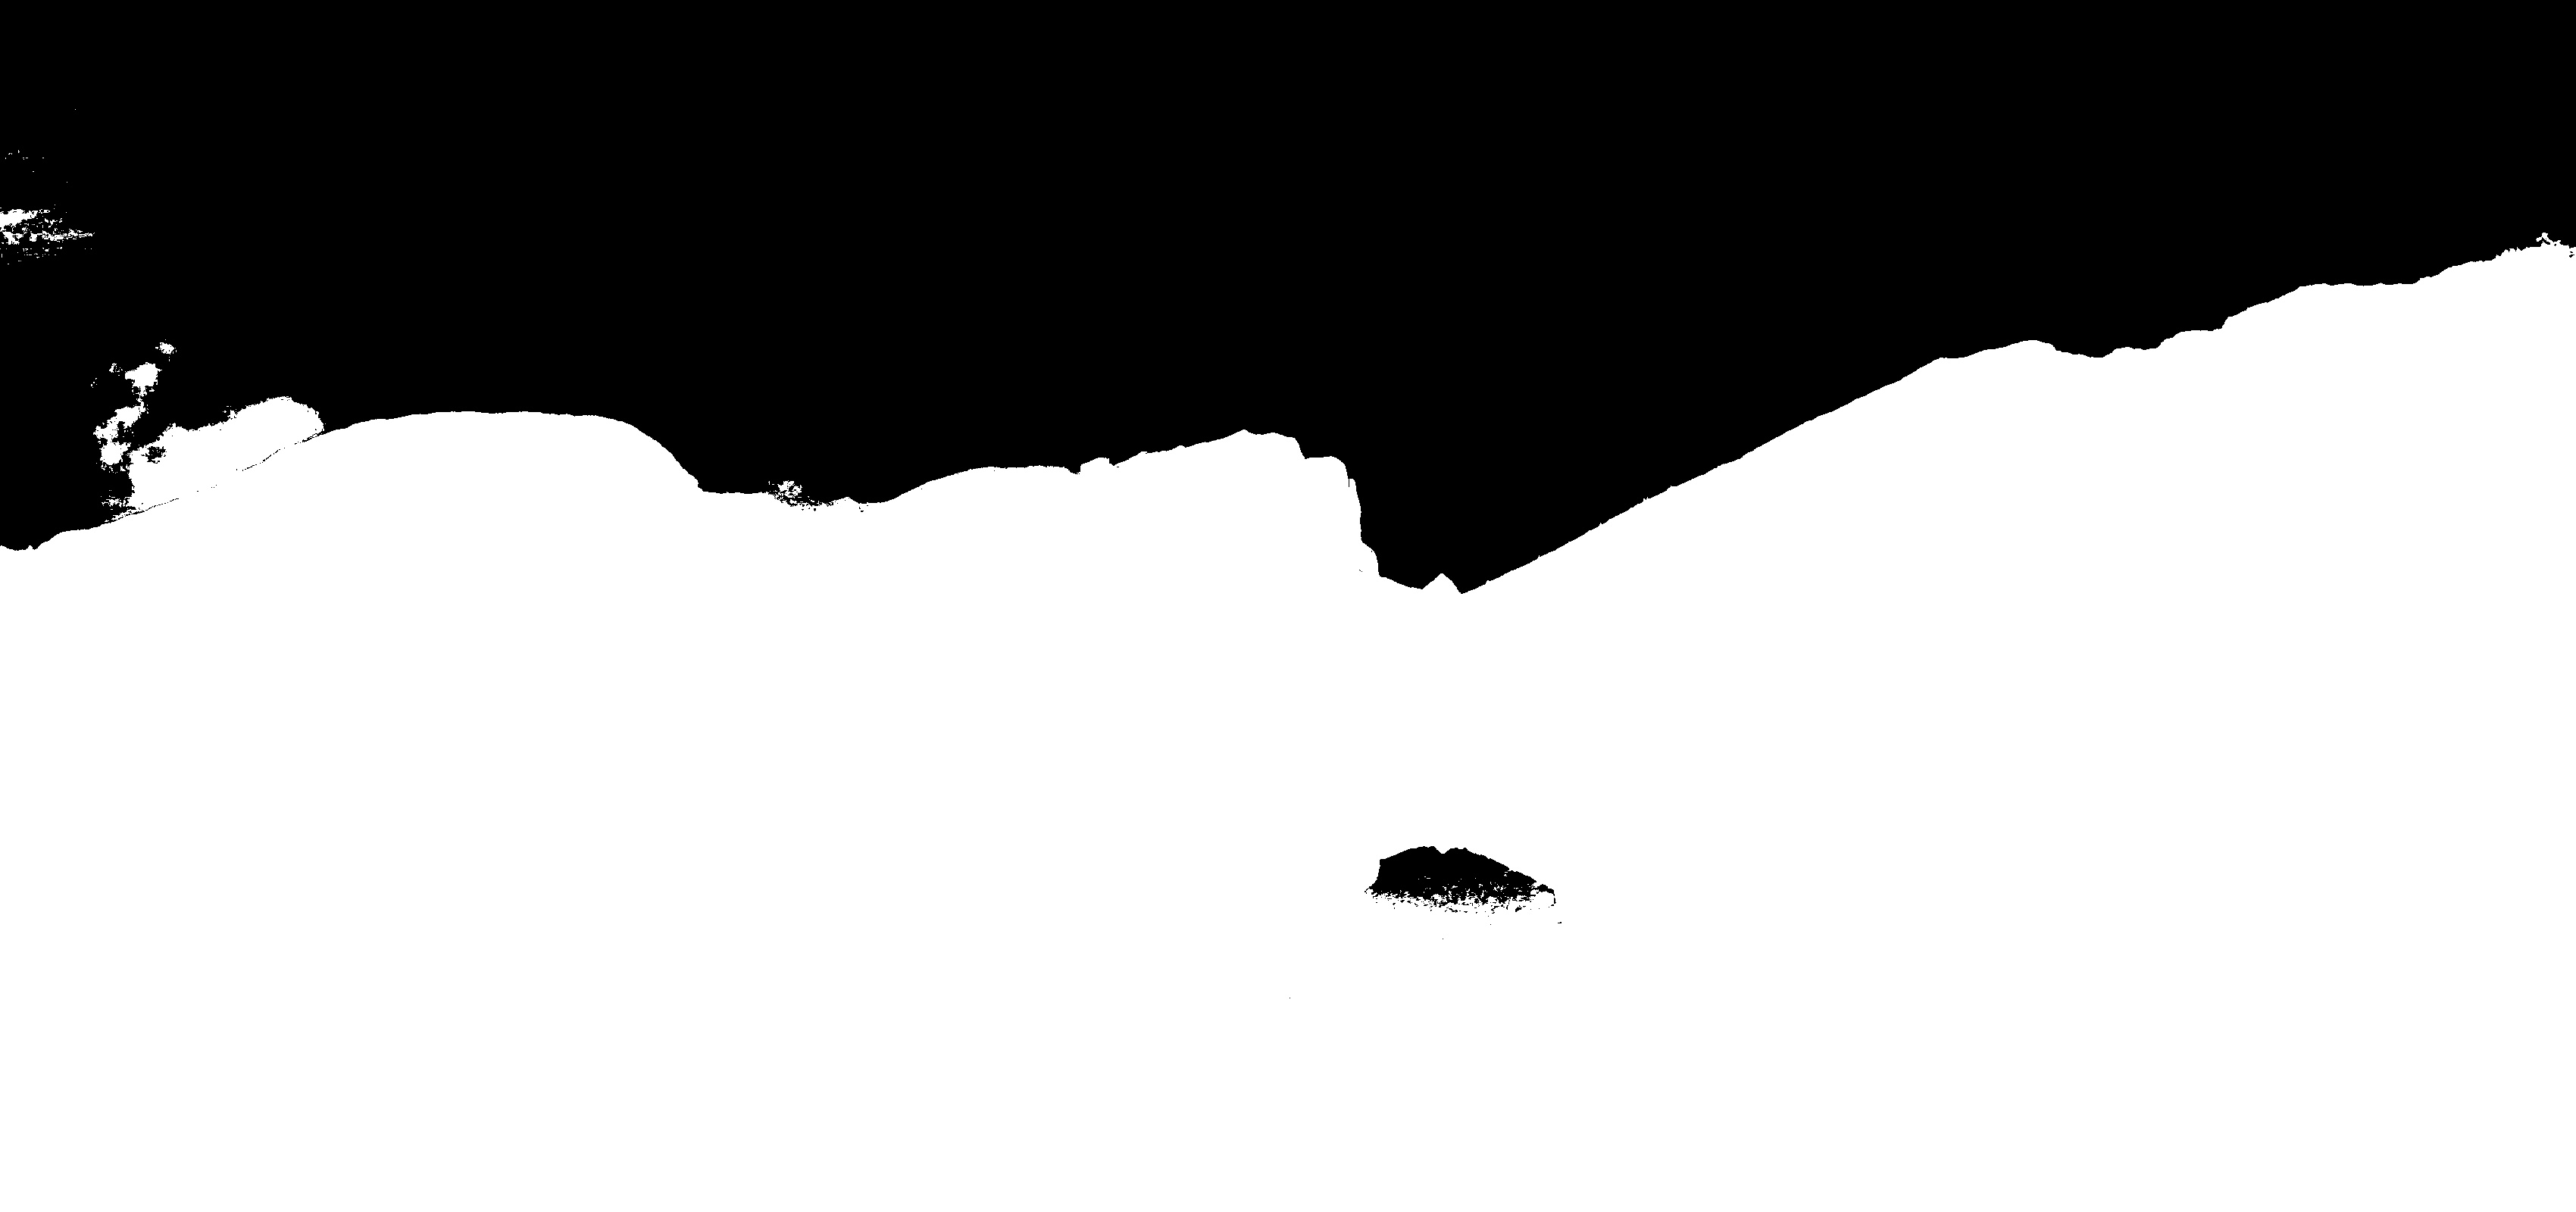
\includegraphics[width=\textwidth]{../Bilder/Sky_Blackening_SecondStep.jpg}
\subcaption{Bildmaske}
\label{simg:Alle_Mask}
\end{subfigure}
%
\begin{subfigure}[c]{0.49\textwidth}
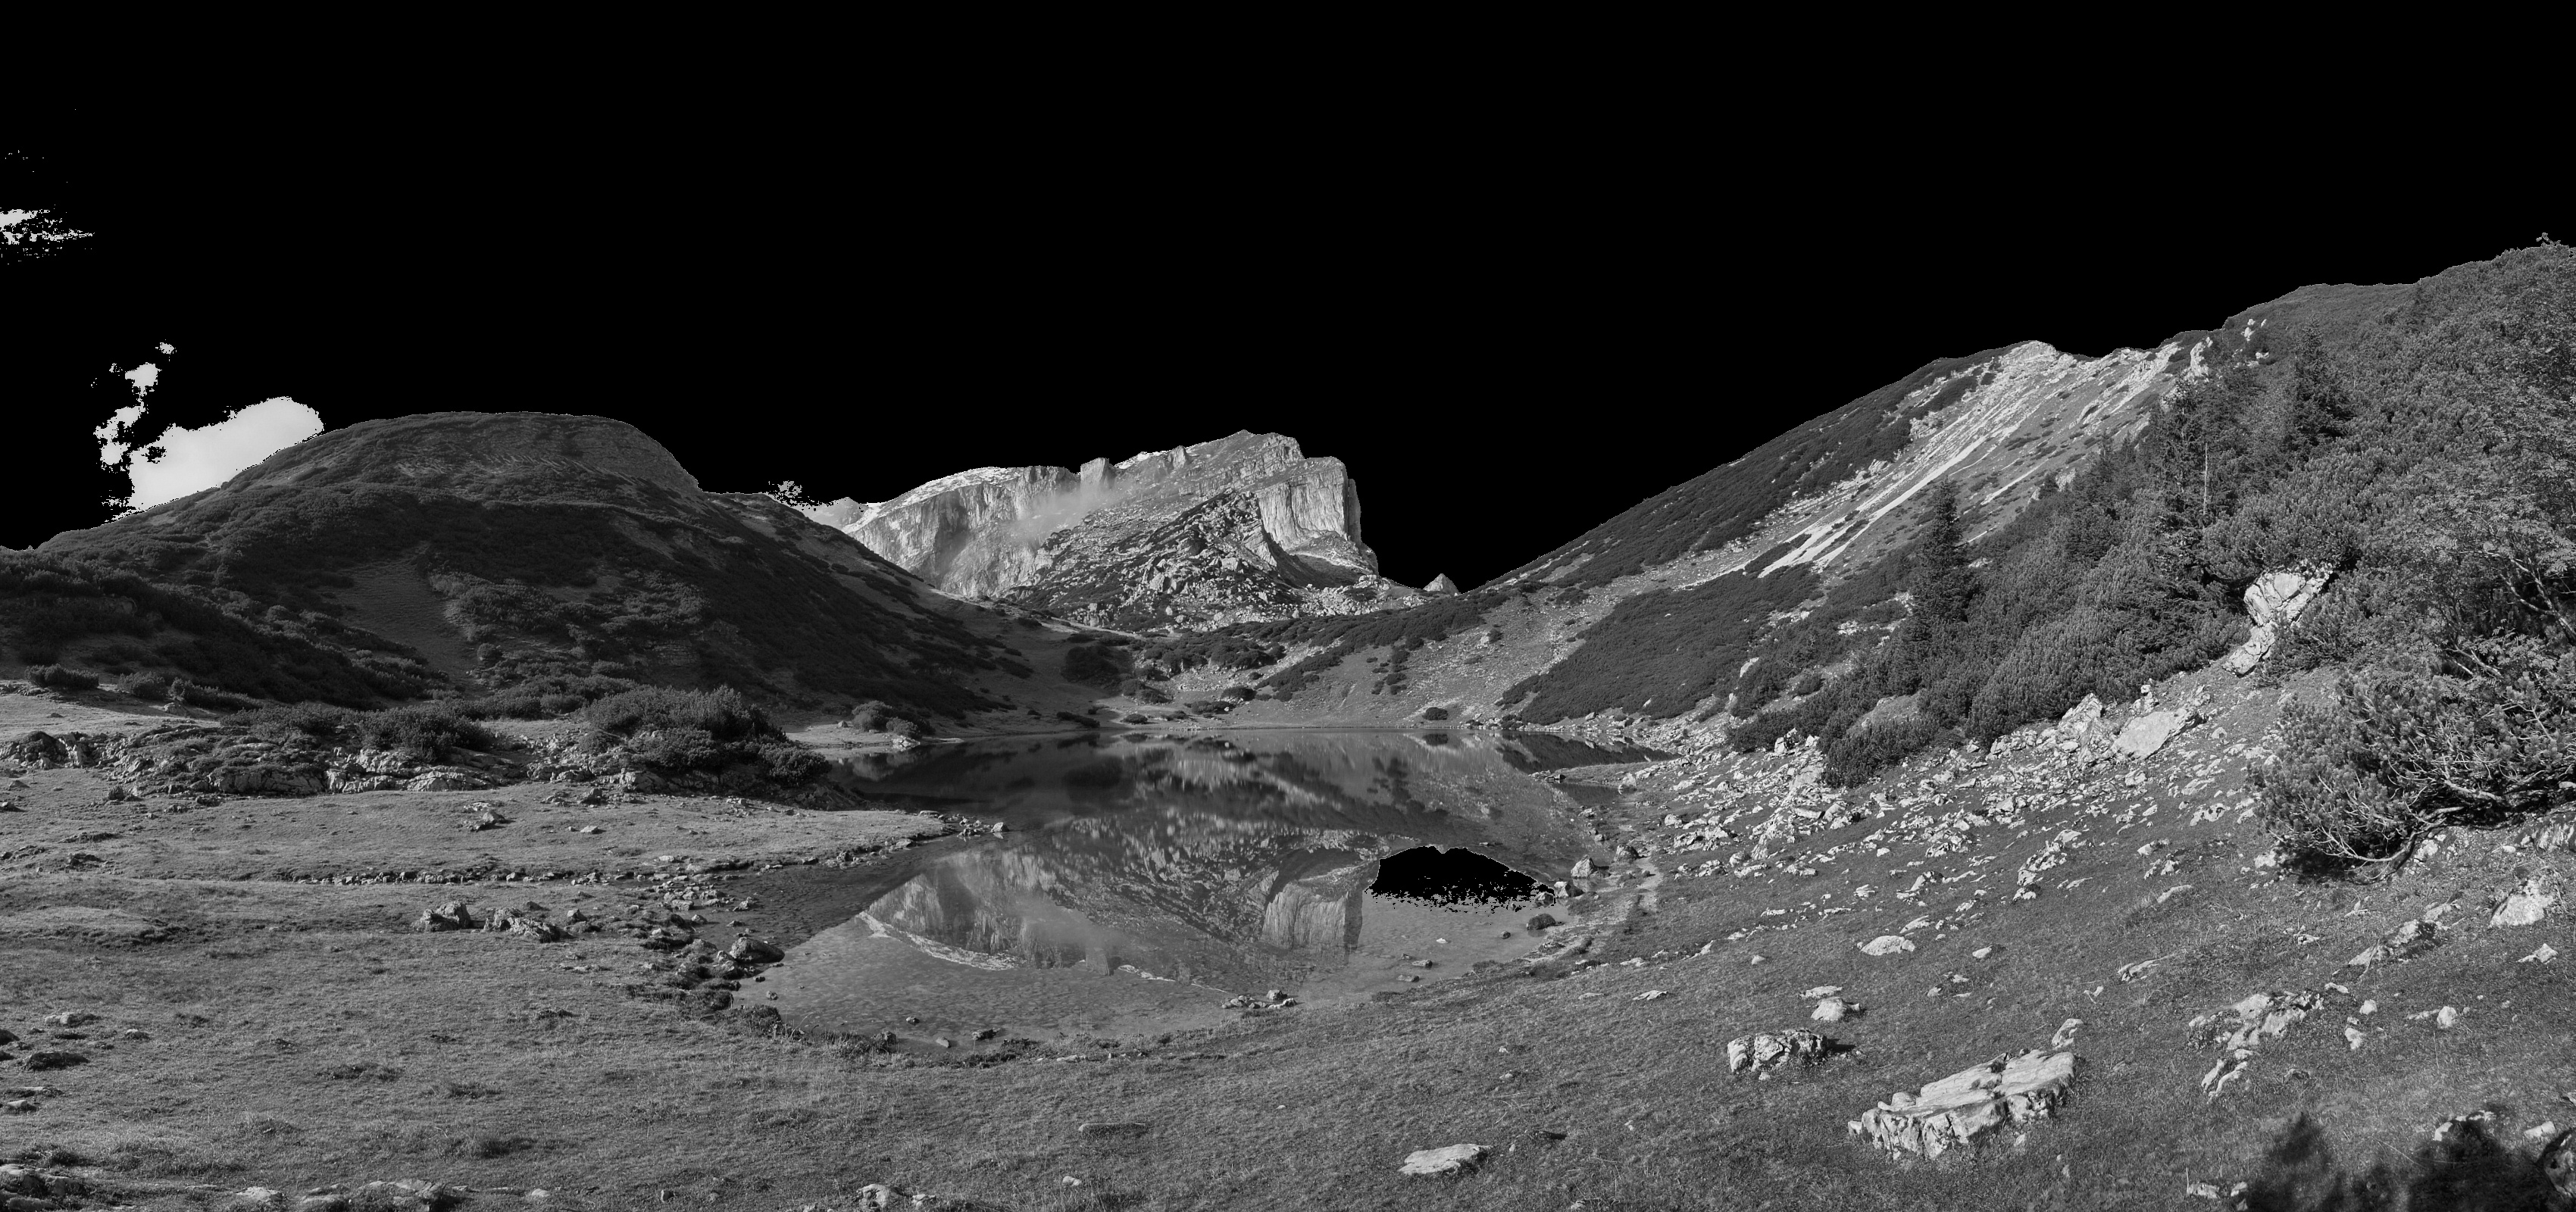
\includegraphics[width=\textwidth]{../Bilder/Sky_Blackening_ThirdStep.jpg}
\subcaption{Bild mit eingeschwärztem Himmel}
\label{simg:Alle_sky_black}
\end{subfigure}
\caption[Kontrasttransformation für sky blackening]{Die vier Transformationsschritte vom Originalbild (a) bis zum Grauwertbild mit eingeschwärztem Himmel (b)}\label{img:Alle_Trans}
%\vspace{-0.3 cm} % Abstand Bild -- Bildbeschriftung
\end{figure} 

Durch das Verfahren wird relativ zuverlässig der Himmel vom restlichen Bild separiert und eingeschwärzt. In obigem Beispiel ist allerdings zu sehen, dass Bereiche des Sees fälschlicherweise dem Himmelzugeordnet werden, während eine der Wolken nicht komplett geschwärzt wird. Diese falschen Segmentierungen machen jedoch nur einen kleinen Anteil des Bildes aus, weswegen ihr Einfluss auf das matching-Ergebnis nicht allzu hoch ist. Trotzdem sollten diese Bilder nicht an Seen oder Landschaften mit sehr hellen Flächen verwendet werden, da sonst zu viele Bildinformationen fälschlicherweise eingeschwärzt werden. Das so erhaltene Grauwertbild wird anschließend wie zuvor vorverarbeitet und gespeichert. Auf diese Weise wird mit allen Bildern der Datenbank und der Datensätze verfahren, vorausgesetzt sie erfüllen die bereits erwähnten Bedingungen. 

Was muss in diesem Kapitel behandelt werden? welche Änderungen sollten Erwähnung finden?
\begin{itemize}
\item Anpassung an die Live-Anwendung durch dynamische Matrix-Erzeugung --> Nacheinander Differenzenvektoren erzeugen und daraus eine Matrix bilden  \cmark
\item Änderung der Matching-Geraden (statt 10 Bilder in der Vergangenheit zu matchen, wird jetzt das aktuelle Bild gematcht)   \cmark
\item Feste Speicheralloquierung für die Matrix (Festlegen der gespeicherten, maximalen Sequenzlänge)   \cmark
\item variable Anpassung der Sequenzlänge (wenn kein Match gefunden wird, wird die Sequenzlänge nach und nach erhöht, um vielleicht doch noch einen Match zu finden)   \cmark
\item Installieren einer Omni-Kamera um die Blickwinkelabhängigkeit zu reduzieren (Wird in biologisch inspirierte Navigation verschoben) \xmark
\item sky-blackening hinzufügen, um Bilder einander anzugleichen   \cmark
\item Suchbereich in der Matrix nach gefundenem Match einschränken (Risiko falsche Matches zu finden wird deutlich reduziert)   \cmark
\item Ändern der Aufnamefrequenz bei fehlgeschlagener Lokalisierung \xmark
\end{itemize}
\pagebreak
\section{Biologisch inspirierte Navigation}
Für die autonome Navigation eines Fahrzeugs muss nach der erfolgreichen Lokalisierung eine Kursvorgabe erfolgen. Im Fall des route"=followings bedeutet das eine Richtungsvorgabe um die vorgegebene Route nicht zu verlassen. Weicht das Fahrzeug trotzdem einmal von der Route ab muss der Algorithmus vorgeben in welche Richtung diese liegt, damit das Fahrzeug dorthin zurückkehren kann. 

Normalerweise werden für eine optische Navigation 3D"=Informationen oder sehr hoch auflösende 2D-Kameras benötigt. Aufgrund der hohen Komplexität der derart gewonnenen Daten und den sehr aufwendigen Umrechnungen, steigt die Rechenleistung auf ein beinahe nicht mehr zu bewältigendes Pensum an. Dadurch müssen entweder große Computer auf dem Fahrzeug mitgeführt werden, was das Gewicht steigert und den Energieverbrauch extrem steigert. Oder das Fahrzeug muss ständig mit einem externen Rechner, der die Navigation übernimmt, kommunizieren, wodurch die Reaktionszeit stark erhöht wird. 

Im Lauf der Jahre haben Lebewesen jedoch zuverlässige und gleichzeitig einfache Verfahren zur Lösung dieses Problems entwickelt. Insekten wie die Ameise können beispielsweise Navigationsaufgaben sehr effizient lösen, für die mit modernster Technik Supercomputer benötigt werden würden. Dafür benutzen sie unter anderem optisch gewonnene Informationen. Diese Tatsache ist besonders beeindruckend, wenn man bedenkt, dass die Augen einer Ameise relativ schlecht auflösende Bilder bereitstellen und die Gehirnkapazität im Vergleich zu anderen Lebewesen sehr gering ist. Werden diese Tatsachen auf eine technische Ebene transformiert, bedeutet das eine sichere und zuverlässige Navigation mit niedrig auflösenden Bildern, bei gleichzeitig sehr geringem Speicher"= und Rechenbedarf.

Diese Vorteile haben bereits viele Untersuchungen angeregt, deren Ziel eine technische Umsetzung des Navigationsalgorithmus' von Ameisen ist. Nachdem zuerst kurz die Vorgehensweise des biologischen Originals beschrieben wurde, soll die für den SequenceSLAM angepasste Implementierung ausführlich erläutert werden. 
\subsection{Navigation der Ameise}
Ameisen besitzen, wie die meisten anderen Insekten einen dreigeteilen Körper, wobei der Kopf kein eigenes Drehgelenk besitzt. Das bedeutet, dass die Ameise immer in die Richtung blickt, in die sie sich gerade bewegt. Zudem besitzen sie Facetten"= oder sogenannte Komplexaugen, die einen Blickwinkel von beinahe $360^{\circ}$ ermöglichen. Die Auflösung dieser Bilder ist jedoch, wie bereits erwähnt, vergleichsweise gering. 

Für den ersten Lauf zu einer Futterquelle markieren sich die meisten Ameisenarten die gelaufene Route mit einer Pheromonspur. Jedes Mal, wenn sie anschließend die Strecke wiederholt, folgt sie dieser Spur und merkt sich parallel die Umgebungsbilder. So kann sie auch noch nach mehreren Tagen, wenn längst keine Duftstoffe mehr ihren Weg markieren, diesen sehr präzise anhand der optischen Informationen wiederfinden. 

Dabei nutzt sie, dass ihr Kopf, und damit das Bild der Umgebung, immer in die aktuelle Bewegungsrichtung zeigt. Um herauszufinden, in welche Richtung sie nun weiterlaufen muss, dreht sie ihren Körper ein wenig nach links und nach rechts. Anschließend entscheidet siein welche Richtung das Bild am ähnlichsten mit einem der gemerkten Bilder aus der \glqq Datenbank\grqq{ }war und setzt ihren Weg dorthin fort. 
%Einfügen von Bild einer Ameise und drei Blickwinkel, in die sie sich bewegen kann
\begin{figure}[h!]
\centering
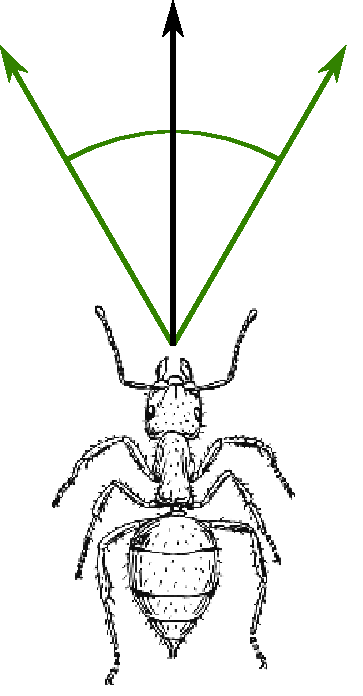
\includegraphics[width=0.3\textwidth]{../Bilder/blickwinkel_aenderung.pdf}
\caption[Wegfindung der Ameise]{Schematische Darstellung der Wegfindung von Ameisen. In diesem Beispiel wird aus drei Richtungen die weitere Bewegungsrichtung der Ameise gewählt.}
\label{img:Am_Blick}
\end{figure} 

Ein weiterer Aspekt ist das Erreichen des Endpunktes. So kann es durchaus einmal passieren, dass die Ameise an ihrem Nest oder dem Futterplatz vorbeiläuft. Um dies und eine damit einhergehende Orientierungslosigkeit zu verhindern, läuft sie den Endpunkt einmal aus allen Himmelsrichtungen ab. Dabei merkt sie sich die Umgebung aus allen möglichen Blickwinkeln, um so zum Nest zurückzufinden, sollte sie einmal vorbeigelaufen sein \cite{baddeley2012model}. 

Die aufgenommene Route ist nicht bidirektional. Kennt also die Ameise den Weg vom Nest zum Futterplatz, kann sie deswegen nicht automatisch entlang der gleichen Strecke zurück laufen. Daher können die Hin"= und die Rückroute durchaus unterschiedlich sein. 

Der gesamte Prozess lässt sich aufgrund seiner Einfachheit und Schnelligkeit perfekt mit dem SequenceSLAM kombinieren. Hierbei findet die Lokalisierung mithilfe des SequenceSLAM statt und anhand der Rotation des Bildes soll anschließend ein Zurückfinden auf die Route ermöglicht werden, sollten einmal Abweichungen vorkommen. Die genaue Implementierung in den Algorithmus wird im Folgenden Kapitel beschrieben.
\subsection{Technische Umsetzung}
Für die Anwendung der Navigation der Ameise im SequenceSLAM mussten sowohl Hardware, als auch Software angepasst werden. Bei der Hardware handelte es sich vor allem um die Kamera, die zur Aufnahme verwendet werden sollte. Vorher wurde eine Kamera mit einem Öffnungswinkel von $90^\circ$ in der Höhe und Breite verwendet. Diese besaß den Nachteil, dass das Fahrzeug selbst oder eine Pan-Tilt Einheit unter der Kamera gedreht werden mussten, um die Umgebung aufzunehmen. Das kostet Zeit und macht den Algorithmus undynamisch, da das Fahrzeug an jedem Aufnahmepunkt stehen bleiben müsste, um die weitere Bewegungsrichtung zu ermitteln.

Aufgrund der Empfindlichkeit gegenüber kleinen Verschiebungen der Kameraposition und der Blickwinkeländerung, hat der reine Grauwertvergleich zudem Schwierigkeiten einen guten Match bei verschiedenen Rotationen zu finden. Dies kann nur dann gelingen, wenn nach einer Rotation um einen bestimmten Winkel diese beiden Parameter in der Realität und im Datenbankbild genau gleich sind. Da solche Treffer in einem realen, physikalischen System beinahe unmöglich sind, muss vor der eigentlichen Implementierung der Navigation die Unabhängigkeit des Matchings gegenüber Positions"= und Blickwinkelschwankungen sichergestellt werden.

Der Algorithmus ist dabei gegenüber allen drei Rotationen, also yaw, pitch und roll, empfindlich. Zudem haben Verchiebungen entlang der y- und z-Achse des Fahrzeugs großen Einfluss auf das Matching. Verschiebungen entlang der x-Achse des Fahrzeugs sind jedoch differenzierter zu betrachten. Im Normalfall handelt es sich hierbei um Positionsänderungen entlang der Route, deren Einfluss maßgeblich vom metrischen Abstand zwischen den einzelnen Bildern in der Datenbank und der Größe der aufgenommenen Szenerie abhängt. 

Sind die Abstände zwischen den Bildern im Vergleich zur Größe der aufgenommenen Landschaft sehr groß, können Verschiebungen entlang der x"=Achse um die aktuelle Datenbankposition zu Problemen beim Matching führen. Dabei werden unter Umständen komplett andere Szenerien aufgenommen, die keine Ähnlichkeit zu einem der Datenbankbilder besitzen.
%Einfügen von Nordland-Bildern großer Abstand

Im Gegensatz dazu können kleine Abstände zwischen den Bildern im Vergleich zur Größe der aufgenommenen Landschaft, ändern sich die Bilder bei Verschiebungen nicht so stark. Sollte die Verschiebung größer als der Abstand zwischen zwei Bildern sein, ist der beste Match beim vorherigen oder nachfolgenden Bild. 
%Einfügen von Nordland-Bildern kleiner Abstand

Für diese Arbeit wird davon ausgegangen, dass die Abstände im Vergleich zur Größe der aufgenommenen Szenerie relativ gering sind. Daher erübrigt sich die Implementierung einer Unabhängigkeit gegenüber Verschiebungen in der x"=Achse.
\subsubsection{Installation einer Omni-Kamera}
Die erste Maßnahme, um die Blickwinkelunabhängigkeit bei der Aufnahme zu erhöhen, war die Verwendung einer Omni-Kamera. Im Gegensatz zu herkömmlichen Kameras können mit ihr $360^\circ$ Aufnahmen für den Algorithmus bereitgestellt werden. Die Bilder der Kamera werden auf eine \glqq Kugel\grqq{ }oder einen \glqq Zylinder\grqq{ }projiziert. Anschließend werden die Bilddaten mithilfe von Umrechnungen der Oberflächen in ein Rechteck in ein 2D"=Bild umgewandelt. Die so gewonnenen Bilder werden dann wieder für den SequenceSLAM in einem Bildvektor gespeichert.

Aufgrund dessen, dass nun der komplette Bereich um die Kamera herum aufgenommen wird, wird das Bild komplett unabhängig gegenüber Drehungen um die z"=Achse der Kamera. Weisst ein Bild eine yaw"=Rotation zum ursprünglichen Bild auf, kann programmatisch eine Drehung des Bildes simuliert werden. Hierfür wird die Breite des Bildes durch $360$ geteilt, damit man die Skalierung des Bildes in Pixel pro Grad erhält. Diese wird daraufhin mit der benötigten Rotation multipliziert. Die so berechnete Anzahl an Pixeln wird dann anschließend vom linken oder Rechten Rand abgeschnitten und an den gegenüberliegenden Rand angefügt. Dadurch wird bildlich gesprochen die vorher gewählte Schnittkante um einen bestimmten Winkel verschoben.
%Bilder aus der Simulation mit Omni-Cam (eins normal, eins gedreht)

Wenn die z"=Achse des Fahrzeugs und der Kamera gleich sind, sind die Bilder auch gegen Fahrzeugrotationen auf der Stelle unabhängig. Das bedeutet, dass das Verwenden einer Omni"=Kamera die Empfindlichkeit gegenüber yaw"=Rotationen komplett entfernt. 

Desweiteren wird durch die Omni-Kamera die Abhängigkeit gegenüber Verschiebungen in der y"=Achse verringert. Bei einem normalen Bild gehen Bildinformationen bereits bei sehr kleinen Verschiebungen an der einen Seite verloren, während an der anderen Seite welche hinzukommen. Gerade der reine Grauwertvergleich hat dann Schwierigkeiten, da die Positionen der zueinanderpassenden Pixel komplett verschoben sind. 
%Nordland-Bild mit Verschiebungen

Zwar besteht dieses Problem bei einer Omni"=Kamera auch, aber nur in der Richtung orthogonal zur Bewegungsrichtung. Hier findet die größte Änderung statt, auch schon bei kleinen Verschiebungen. In der Bewegungsrichtung ändert sich das Bild jedoch kaum. Hier greift der gleiche Effekt, der vorher bei der x"=Achsenverschiebung auftrat. Das bedeutet, dass sich die Pixel in der Verschiebungsrichtung nicht so stark ändern. 

Dadurch können die relativ großen Änderungen entlang der zur Verschiebung orthogonalen Bildachse durch die wenigen Änderungen entlang der Verschiebungsrichtung relativ gut ausgeglichen werden. Zudem kann auch hier das Bild wieder auf der Stelle rotiert werden. Auf diese Weise können bei kleinen Verschiebungen die Pixel wieder ansatzweise an ihre richtige Position geschoben werden. Somit werden die Unterschiede aneinander angeglichen. Anstatt stellenweise sehr große und sehr kleine Unterschiede zu haben, werden die Pixeldifferenzen überall relativ moderat. So können kleine Abstände von der zwischen der aktuellen Position und der ursprünglichen Aufnahmeposition ausgeglichen werden.

Allerdings kann durch eine Omni"=Kamera nicht die Verschiebung entlang der z"=Achse der Kamera ausgeglichen werden. Auch der Neig"= und Schwenkwinkel haben noch einen großen Einfluss auf das Matching"=Ergebnis. Bei Bodenfahrzeugen, die in Gebäuden unterwegs sind, sind diese Parameter irrelevant, da solche Verschiebungen nur in einem sehr geringen Maß auftreten. Für andere Anwendungen kann noch ein sogenannte gimbal verwendet werden, der die Kamera immer entlang der xy"=Ebene ausrichtet. Dadurch hätten der Neig"= und Schwenkwinkel ebenfalls keinen Einfluss mehr auf die Vergleichsergebnisse. Nur die Verschiebung entlang der z"=Achse kann nicht hardwaretechnisch kompensiert werden. Da für den SequenceSLAM bisher jedoch nur Boden"=Fahrzeuge verwendet wurden, kann dieser Aspekt zunächst vernachlässigt werden.
\subsubsection{Einbindung der biologischen Navigation in den SequenceSLAM}

Was muss in diesem Kapitel erwähnt werden? Wie ist der Aufbau?

\begin{itemize}
\item Navigation von Insekten anhand der Paper von Wolfgang --> Was gehört dazu?
\begin{itemize}
\item Drehen des Kopfes und Bewegung in die Richtung mit höchster Übereinstimmung aus der Datenbank
\item Durch Verwenden einer Omni-Kamera präzisere Lokalisierung möglich
\item Omni-Kamera erhöht zudem den Abweichungswinkel
\end{itemize}
\item Ermitteln der Rotationswinkel aus dem Panoramabild --> Beispiele mit Landmarken an verschiedenen Positionen
\begin{itemize}
\item Vorne und hinten separat matchen
\item Gesamtes Panoramabild drehen und besten match suchen
\item Vor- und Nachteile der beiden Methoden
\end{itemize}
\item Kurskorrektur on the fly, also ohne das Fahrzeug unnötig abzubrechen. Ausnahme: Abweichung von der Route ist zu groß --> stehen bleiben und Fahrtrichtung korrigieren, um zu große Abweichungen zu vermeiden.
\end{itemize}
%Danach kommt das biologisch inspirierte Verfahren zum Zurückfinden auf die Route dran. Für diesen Teil sollten vermutlich etwa 10 bis 20 Seiten verwendet werden. 
\pagebreak
\section{Versuchsaufbau und -durchführung}
%Hier wird der genaue Versuchsaufbau und die anschließende Durchführung genau beschrieben. 
\pagebreak
\section{Ergebnisse und Evaluierung des Verfahrens}
%Zum Schluss kommt die Evaluation, die Testergebnisse und noch ein Ausblick. Auch hier: 10 bis 20 Seiten
%Zur Bewertung: Es müssen 10 Bilder aufgenommen werden, bevor ein sinnvolles Matching möglich ist.
\pagebreak
\section{Ausblick}
\pagebreak
\renewcommand{\refname}{Quellenverzeichnis}
\bibliography{Bachelorarbeit}
\bibliographystyle{ieeetr}

\end{document}